\documentclass[conference]{IEEEtran}

\usepackage{cite}
\usepackage{amsmath,amssymb,amsfonts}
\allowdisplaybreaks
\usepackage{algorithmic}
\usepackage{graphicx}
\usepackage{textcomp}
\usepackage[dvipsnames]{xcolor}
\usepackage{hyperref}
\usepackage{booktabs}
\usepackage{pgfplots}
\usepackage{braket}
\usepackage{upgreek}
\usepackage{mathtools}
\usepackage{caption}
\usepackage{cuted}


\def\BibTeX{{\rm B\kern-.05em{\sc i\kern-.025em b}\kern-.08em
    T\kern-.1667em\lower.7ex\hbox{E}\kern-.125emX}}


\pgfkeys{/pgf/number format/.cd,1000 sep={\,}}

\begin{document}

\title{Understanding and Simulating Quantum Circuits}

\author{\IEEEauthorblockN{Shane B.}
shane@wander.dev
}


\maketitle

\pagestyle{plain}


\begin{abstract}
In this paper we present and clarify the mathematical model behind the tool that we
have designed for the purposes of simulating quantum computations using the circuit model, through means of an UI-based
user interface running on a general-purpose, classical computer (PC).
The aims are (1) to provide a high-level overview of the field;
(2) explain the basic theoretical concepts as they are implemented in the current version of our tool at this time;
(3) provide several visual demonstrations and explanations of simple quantum algorithms, recreated using our UI tool.
\end{abstract}

% the first section provides the context for your work and describes the structure. Be sure to formulate your most
% relevant research questions (also important for your poster !). Have a look at the guidelines for additional tips.

\section{Distinguishing Characteristics of Quantum Computing}

\label{sec:theQuantumModel}

Our physical world can be described and predicted using quantum mechanics.
In comparison to classical physics, quantum mechanic posits a \textit{probabilistic model} in which we work with the \textit{probability} of an entity being in a given
\textit{state}.
In this model, on top of allowing a single concrete state like the binary model (exactly 0 or exactly 1) of classical computing,
in certain situations in a certain sense, we can interpret a \textit{physical entity}
to be in multiple states ``simultaneously''.
And through the application of so-called \textit{operators}
we are able to compute some interesting results directly and instantaneously by leveraging the rules of our reality.
Let us introduce the quantum version of \textit{state} through the well-known \textit{Schrödinger's Cat} thought experiment,
in which we can consider the cat to have a ``state of liveness''.
We can use its ``liveness'' to represent our ``\textit{qubit}'' (for \textit{``qantum bit''}) which we denote $q_{cat}$.
Initially, the cat is alive, and hence $q_{cat} = 1$ with
a 100\% probability ($p_{alive} = 1.0$).
Subsequently, the cat is placed in a box with a radioactive source. Then, per \textit{quantum mechanics},
the source may or may not cause the cat to die, both with \textit{equal probability}.
In the death outcome, which has a probability $p_{dead} = 0.5$, this would result in a final state $q_{cat} = 0$.
The alive outcome has $p_{alive} = 0.5$, and would result in a final state $q_{cat} = 1$.
Before we \textit{observe} the cat in the box to determine the actual outcome,
the cat's state is in \textit{quantum superposition} meaning it can be interpreted as being ``dead'' and ``alive'' simultaneously.
Upon \textit{observation} (or \textit{measurement}) of the outcome, we will find one of the two definite
results, the probability of both given by the probability distribution $\left[p_{dead}\ p_{alive}\right]$.
In quantum mechanical terms, it is said that \textit{measurement}
results in the \textit{collapse of the wave function}, which produces a \textit{definite state}.
In the quantum computing, physicists will opt to use simpler entities (\textit{particles} in particular) to represent \textit{qubits}, such as for
example \textit{encoding} our qubit state using the orientation of electrons or photons.


A next important quantum mechanical feature for the purposes of achieving computationally interesting results,
is that we can take any $n$ such qubits and ``link'' any two or more of them together
(\textit{entangle} them), such that when the state of one of the qubits is manipulated,
the state of the other will \textit{simultaneously} change in a predictable way
in turn.
Once two qubits are entangled, this simultaneous synchronised effect continues to
operate at a potentially large distance — this effect being what Albert Einstein described as ``spooky action at a distance'' \cite{ref:nobel2022phys}.
The \textit{entanglement} is preserved until measurement of any of the involved qubits, upon which a single definite result for all involved qubits
is produced and any trace of the entanglement is destroyed. This is notably different from the behaviour of bits in classical computers,
where a similar ``manipulation'' would strictly need to be performed in a ``separate step'' for each bit,
such as in a classical sequential algorithm or a classical parallel electronic circuit needing to manipulate both bits
using separate logic gates (Appendix \ref{appendix:OverviewClassicalStateMgmnt}, Figure \ref{fig:bitflipcodeblock} \& \ref{fig:setofnotgates}).

The final and truly novel property of quantum mechanics is that —
on top of directly providing the ``randomness'' required for \textit{probabilistic computing} —
it enables us to directly work with \textit{complex numbers} in computing our state-probabilities.
The probabilities of states are encoded in complex numbers (called \textit{amplitudes}) and these \textit{decode} to non-complex \textit{probabilities}.
Through creative applications of \textit{operators}, complex numbers allow us to achieve interesting
effects in our computations, such as allowing the "cancelling" of the probability of select states being true,
which would not have been possible solely using probability theory\cite{ref:quantumcomputingsincedemocritus}.


The \textit{Quantum} model of computation, then, is built on the idea of directly leveraging these interesting properties of the physical, quantum mechanical world
we inhabit exploiting them to the benefit of our physical hardware and algorithms,
expanding upon what we can directly compute with classical bits.
Within this system, a single \textit{``quantum algorithm''} for solving a specific computational problem encompasses: a particular number $n$ of \textit{qubits};
their initial \textit{states} (or values); and the \textit{operations} performed on the qubits in a well-defined order,
which determine the final
\textit{probability distribution} for the final states of the qubits, right before \textit{measurement}. A \textit{``quantum computer''}
respectively denotes the combination of all such hardware components necessary execute a quantum algorithm.
There are various means of representing a quantum algorithm. The most common of such is the \textit{``quantum circuit''}
\cite{ref:ibmqiskitdocs,ref:microsoftquantumdocs,ref:googlecirqdocs}, which is the subject of the tool discussed in this paper.


\section{Anticipated role in Computer Hardware Architecture Model}

The ultimate purpose of quantum computing is to leverage the properties of our quantum mechanical world as a ``shortcut'' to achieve more efficient computations for certain problems.
Quantum computers would not necessarily enable us to compute anything ``new'' — in the sense that any algorithm we may design using quantum computers can also be
performed using a classical computer, though perhaps less efficiently. Any quantum computer is Turing-Complete
\cite{ref:quantumvialinearalgebra}, hence is able to execute any classical computer algorithm.

A likely application of quantum computers in our theoretical model of what makes a modern computer would not be to replace classical computers
as we currently know them, but as a module within a classical computing system, similar to the
\textit{FPU}\cite{ref:wikipediaFPU} or \textit{GPU}.
GPUs are a relevant comparison, as they are optimized for the specific problem of \textit{parallel computation}
and are \textit{programmable}, enabling \textit{parallel computing algorithms} within their own specific paradigm \cite{ref:nvidiacudamanual, ref:amdromconlinedocs}.

In the future, provided we can solve the challenging problem of physically engineering a quantum computer that can accurately reflect the theory,
as we have achieved with silicon semiconductor chips
 — which is an active area of research \cite{ref:quantumcomputers2023article} —
then we may find ourselves in a world where quantum computers
are used as designated and programmable \textit{key components} within various classical computer systems — called a \textit{QPU} (\textit{Quantum Processing Unit}) \cite{ref:wikipediaQPUlist}.

\section{Real-World Applications}

On a high level, we can distinguish about three broad categories of applications for quantum computing technology.
These categories may not be exhaustively representative of all current areas of research.

The first and most obvious use-case for quantum computers is modelling physical and chemical processes directly.
Currently, physicists and chemists trying to model large,
complex systems within their domains are required to translate said processes in classical
computing terms. Often these relations cannot be expressed directly in classical terms, and need to be approximated when converted to classical computing terms.
Hence, the quantum mechanical interactions between the objects within some of these processes also have to be computed in classical terms.
All these translations form layers of overhead that become incredibly slow at scale,
such that in many cases the scientists are required to either use smaller models
instead of accurately large ones (which do not produce as accurate results) or depend on expensive supercomputers
(which are only helpful up to a point, for very large systems of objects).
In such cases, quantum computers would provide a benefit even without needing to consider any complex \textit{quantum algorithms},
as enabling such scientists to model their problem directly \textit{alone} would serve as a large
improvement, having a direct impact on commercial areas of research such as material discovery and drug development \cite{ref:bova2021commercial}.


Secondly, the next category consists of use-cases leveraging quantum computers in combination with the
advanced \textit{quantum algorithms} they would enable. %, particularly within various STEM and STEM-adjacent fields.
One example of a paradigm-shifting algorithm is
\textit{Shor's Algorithm for Prime Factoring} \cite{ref:shorsalgorithm}.
Currently, a lot of public-key cryptographic systems
such as  \textit{Finite Field Diffie-Hellman} \cite{ref:rfc7919},
\textit{RSA} \cite{ref:rsapaper} and
\textit{ECC}\footnote{ECC in particular relying on a method \textit{close} but more difficult than prime factoring,
but which is still reducible to factoring\cite{ref:quantumcomputingsincedemocritus,ref:ellipticcurves1986}}
rely on prime factoring
as their ``mathematically hard problem'' of
choice\footnote{Cryptographic systems will generally be designed around such \textit{hard
problems}: mathematical problems which are easy to solve computationally when sufficient information is known in advance,
but hard to ``brute-force'' without advance knowledge of this key information}.
Classically, our best known means of finding the prime factors
of an arbitrary integer $n$
— the \textit{General Number Field Sieve} algorithm (\textit{GNFS})\cite{ref:wikipediaGNFS} —
has an asymptotic time complexity of $O(e^{1.9(\log{n})^{1/3}(\log{\log{n}})^{2/3}})$.
\textit{Shor's Algorithm} would enable us to compute the prime factors with a \textit{quantum} time
complexity\footnote{A parallel to \textit{quantum time complexity} is the time complexity we compute for \textit{parallel algorithms},
often expressed in terms of the number of processors. \textit{Quantum time complexity} generally doesn't always introduce any new terms, instead simply meaning ``if executed on a quantum computer''}
of $O((\log{n})^2(\log{\log{n}})(\log{\log{\log{n}}}))$ if using \textit{fast multiplication},
or potentially even in $O((\log{n})^2(\log{\log{n}}))$ if using \textit{Harvey and Van Der Hoven multiplication}
\cite{ref:harvey2021integer}.
This drastic reduction in time complexity would render these systems far less secure than expected.
A visual comparison of these time complexities is given in Figure \ref{fig:integerFactoringComparison} of Appendix \ref{appendix:RuntimeComplexityComparison}.
Extensive research has been conducted on alternative ``hard problems''
that are not believed to have any efficient quantum solutions — this is the domain of \textit{Post-Quantum Cryptography} \cite{ref:bernstein2017post}.

Within this category we can also consider \textit{exhaustive searching} (or \textit{function inversion} more broadly),
which classically has a runtime complexity of $O(n)$. Using the quantum \textit{Grover's algorithm} \cite{ref:grover1996fast} we can improve this to $O(\sqrt{n})$.
Outside of obvious database search applications, this algorithm also provides a general asymptotic improvement for optimisation problems.


Finally, among other solutions directly leveraging quantum mechanical properties, and opposite to Post-Quantum Cryptography, we can find \textit{Quantum Cryptography}.
Central to this particular field is \textit{quantum key distribution} (\textit{QKD})
— a protocol that is based on exploiting the fact measuring a quantum superpositon is a destructive operation.
Any attempt to learn (and thus \textit{measure}) a non-basis state will result in a change in the state: a definite value being produced
according to the probability distribution due to \textit{wave function collapse}, with all information regarding the superposition
being ``lost'' at that instant.
This property can be employed to determine if a potential 3rd party attempted
to eavesdrop a ``quantum communication channel'', as the intended recipient
of a ``quantum message'' would then determine that the measurement happened earlier than intended,
and take action to work around the problem \cite{ref:quantumcomputingsincedemocritus,ref:advancesinquantumcryptography2020}.
Further impactful uses for quantum computing are still an open question,
with a lot of investment being made to develop use cases within various domains \cite{ref:xprizeforquantum}.


\section{Why Simulate Quantum Circuits?}
\label{sec:whySimulateQuantumCircuits}


At present, we are not yet close to having quantum computers that accurately
model the theory.
The current ``era'' of quantum computing is generally referred to as the  \textit{noisy intermediate-scale quantum}
(\textit{NISQ}) era \cite{ref:preskill2018quantum}, characterised by quantum processors containing up to $n=1K$ qubits which
are neither \textit{fault-tolerant} nor large
enough to achieve \textit{quantum advantage} (or \textit{quantum supremacy}): the ability to demonstrate their
predicted theoretical time complexity improvement over a classical algorithm for large $n$ in the real world.

Ongoing research into quantum computing currently focuses on two main areas: (1) the physical
implementation of the quantum computing systems, particularly sustaining a theory-consistent state of qubits within arbitrary
environments (e.g. minimizing the need for extreme temperature-controlled environments) and
minimizing ``quantum noise'' \cite{ref:resch2021benchmarking}
and (2) designing algorithms within the theoretical quantum model that exploit the benefits of the
quantum paradigm of computation, which would be theoretically capable of achieving quantum advantage.
The software tool that we have designed would aim to assist in the second of above categories, in that it means to
enable the higher-level design of quantum algorithms, without needing to understand the underlying technology implementing
the quantum computing system on which the algorithm may be executed.


\section{Software Design \& Architecture Summary}

The paradigm of implementation of the quantum circuit design tool was a visual, interactive Graphical User Interface (GUI).
The main distinguishing feature of our tool, compared to %widely-available free and open-source
alternatives such as IBM's Qiskit \cite{ref:ibmqiskitdocs} is the ability to design the circuit interactively, through means of
cursor-based drag-and-drop actions.
Our tool distinguishes itself from Qiskit in particular by avoiding the need to have a working
knowledge of Python nor requiring to write any classical computer code.

We have opted for the Python 3 programming language based on the following of its characteristics:
(1) it being the standard and widely-known scientific programming language of choice;
(2) the OS-independence of the language and its built-in graphical modules;
(3) the ability to easily convert datastructures to other widely-used representations such as Qiskit simply by using their existing Python packages;
and (4) its support by cloud web service providers\cite{ref:amazonawsserverless}, allowing reuse of our common modules if deploying on the cloud.

\begin{figure}[tbp]
\centerline{
    \includegraphics[width=0.5\textwidth]{img/ui_startup.png}
}
\caption{GUI of the Quantum Circuit Designer, on initial startup}
\label{fig:guiToolOnStartup}
\end{figure}

The tool presents the user with a digital ``modelling sheet'' and the \textit{Basic Quantum Gate Library} (``G-Lib'') (Figure \ref{fig:guiToolOnStartup}).
The library can be used to recreate the effects of any complex \textit{quantum gate} that
is not part of the library, through means of composing (or combining) multiple simple gates, similar to how one might represent some
classical logical (binary) gates such as \textit{XOR} using a composition
of \textit{AND}, \textit{OR} and \textit{NOT} gates (see Figure \ref{fig:logicalXORcircuit} of Appendix \ref{appendix:ClassicalLogicGates}).
% The library is described in more detail in section \ref{sec:BasicGateLibrary}.


The code-level implementation of the tool can be described as being composed of two sets of code modules: (1) the
``backend'' module, providing the data structures to represent a quantum circuit design as well as the logic for interpreting
it as the underlying matrix operations it represents, allowing serialisation and deserialization of the data
structures, and computing the final probability distribution; and (2) the ``front-end'' module, supplying the means of rendering the
interactive GUI, applying a user's visual manipulations to the backend data structures,
and facilitating a clear visualisation of resultant probability distribution.

\section{Formal Model: Input and Operations}
\label{sec:MathematicsBehindAQuantumCircuit}

The initial ``input state'' or \textit{input binary string} to a circuit is typically a \textit{basis state}:
a $m=2^n$ element vector to represent the $n$ (qu)bits of the input string.
Inputs are represented using \textit{Bra-ket} notation (also known as \textit{Dirac notation}), which is inherited from the field of physics.
In physics, a ``Ket'' is a $n$-element \textit{complex vertical vector} $\in \mathbb{H}^n$
— that is, it is part of a \textit{complex} Hilbert space rather than just a more ``typical'' vector $\in \mathbb{R}^n$ —
with a notation $\ket{\psi}$. Here, $\psi$ is simply a label, and
in our case will typically be a binary string, as in $\ket{01}$.
A ``Bra'' is the \textit{conjugate transpose}\footnote{For any matrix,
this means we first \textit{transpose} (``mirror'' along the diagonal),
and then apply \textit{complex conjugation} to every element of the matrix ($a + ib$ becomes $a - ib$)}
of the corresponding Ket, and is thus a \textit{horizontal} vector,
written as $\bra{\psi}$.
Bra-ket notation is useful as for large $n$ it allows us to not need to write out a very large vector containing many elements,
particularly exceedingly many 0-elements in $2^n$-sized vectors.
One may consider this notation to be equivalent to a high-level programming language function,
that produces a vector:

\centerline{
    \includegraphics[width=0.5\textwidth]{img/build_a_ket_code_block.png}
}

For \textit{basis states}, the input binary string is ``mapped'' to the vector in a straight-forward way.
Here we provide an example for the binary string ``$\textcolor{blue}{11}$'',
requiring $n=2$ (qu)bits, and representing the number $3$ in binary/base-2.
The blue highlight is used for emphasis.
\begin{center}
    \begin{tabular}{ll}
        \toprule
        Binary string & ``\textcolor{blue}{$11$}'' ($2$ in \textit{base-2})\\
        Nr of qubits & $n=2$ (length of the binary string) \\
        \textit{Ket} representation & $\ket{\textcolor{blue}{11}}$ \\
        Nr elements in vector & $m=2^n=2^2=4$ \\
        \bottomrule
    \end{tabular}
\end{center}
The corresponding vector is constructed by taking a $m=2^n$ element \textit{vertical vector},
initialising all elements to zero, except for the element at the (0-indexed) index corresponding to the binary string,
counted from top to bottom, which is initialised to 1.
Here we do this for index ``$\textcolor{blue}{11}$'' $=3$ and size $m=4$:


\begin{center}
    \begin{tabular}{r l}

        index & vector\\
        $\begin{matrix} 00 \\ 01 \\ 10 \\ \textcolor{blue}{11} \\ \end{matrix}$
        & $\begin{bmatrix} 0 \\ 0 \\ 0 \\ \textcolor{blue}{1} \\ \end{bmatrix} \equiv \ket{\textcolor{blue}{11}}$  \\

    \end{tabular}
\end{center}

Bra-ket notation is often combined with another concept, which is also used by the \textit{operators} discussed later and which is often
omitted in written Bra-ket formulae: that of the \textit{tensor product}
(or \textit{Kronecker product}). A tensor product, typically denoted with the symbol $\otimes$, can be obtained
of two matrices of any size (including vectors, which can be interpreted as matrices which have either only 1 row or 1 column)
as a generalisation of the following:
\begin{equation*}
\begin{bmatrix}
\textcolor{LimeGreen}{1} & \textcolor{orange}{2} \\
\textcolor{PineGreen}{3} & \textcolor{Red}{4}
\end{bmatrix}
\otimes
\begin{bmatrix}
5 & 6 \\
7 & 8
\end{bmatrix}
=
\begin{bmatrix}
\textcolor{LimeGreen}{1}(5) & \textcolor{LimeGreen}{1}(6) & \textcolor{orange}{2}(5) & \textcolor{orange}{2}(6) \\
\textcolor{LimeGreen}{1}(7) & \textcolor{LimeGreen}{1}(8) & \textcolor{orange}{2}(7) & \textcolor{orange}{2}(8) \\
\textcolor{PineGreen}{3}(5) & \textcolor{PineGreen}{3}(6) & \textcolor{Red}{4}(5) & \textcolor{Red}{4}(6) \\
\textcolor{PineGreen}{3}(7) & \textcolor{PineGreen}{3}(8) & \textcolor{Red}{4}(7) & \textcolor{Red}{4}(8)
\end{bmatrix}
\end{equation*}
A more elaborate visualisation of a tensor product is provided in Appendix \ref{appendix:AlternativeVisualTensorProduct}.
One might also write the following, ommitting the $\otimes$ symbol.
This also demonstrates a convenient shorthand for building large input strings
(here vector indices are added to the left):

$
\ket{1}\otimes\ket{0}
\equiv
\ket{1}\ket{0}
\equiv
\ket{1,0}
\equiv
\begin{bmatrix}
0 \\
1
\end{bmatrix}
\otimes
\begin{bmatrix}
1 \\
0
\end{bmatrix}
=
\begin{matrix}
{\scriptstyle 00} \\
{\scriptstyle 01} \\
{\scriptstyle\textcolor{blue}{10}} \\
{\scriptstyle 11} \\
\end{matrix}
\begin{bmatrix}
0 \\
0 \\
\textcolor{blue}{1} \\
0 \\
\end{bmatrix}
\equiv
\ket{\textcolor{blue}{10}}
$

Finally, it is useful to note that all so-called \textit{basis states} are what is defined, in physics,
as \textit{pure states}.
Considering the case of a \textit{single qubit}, the only (standard) basis states are $\ket{0}$ and
$\ket{1}$\footnote{Alternative ``bases'' can be considered, such as a basis of $\{\ket{-},\ket{+}\}$}.
For $n=2$ qubits, the basis states would be a list of \textit{Kets} of all $2^n$ possible binary values $n$ bits can take,
namely $\ket{00}, \ket{01}, \ket{10}$ and $\ket{11}$, which are also all pure states.

The opposite to the aforementioned relation does not hold however: not all pure states are basis states.
Pure states also encompass \textit{superpositons}: these are non-basis states where, for a \textit{single} qubit,
the qubit has a non-zero probability of being in \textit{both} state $\ket{0}$ \textit{and} $\ket{1}$, both probabilities summing to $1$.
Quantum computing algorithms will exclusively work with \textit{pure states}, typically transforming basis
states (classical inputs) into other pure states through the use of operators (usually \textit{quantum logic gates}).

\begin{figure}[tbp]
    \centerline{
        \includegraphics[width=0.275\textwidth]{img/Bloch_sphere.png}
    }
    \caption{The Bloch Sphere\cite{ref:img:TheBlockSphere}}
    \label{fig:blochsphere}
\end{figure}

Owing to the fact that the Hilbert space $\mathbb{H}^n$ is complex,
all pure states of $n$ qubits can be written as a complex \textit{linear combination} of the basis states. In the case of $n=1$ we have:
\begin{equation}
    \ket{\psi} = \alpha\ket{0} + \beta\ket{1} \ \ (\alpha, \beta \in \mathbb{C}) \tag{6.1} \label{eq:purestate1}
\end{equation}

Mathematically, using the definition\footnote{The ``absolute value'' is also known as the ``modulus''. On a complex number $a + ib$, this is $\sqrt{a^2 + b^2}$}
$|x|=abs(x)$, then $\alpha, \beta$ will satisfy $|\alpha|^2 + |\beta|^2 = 1$.
Here, $\alpha$ and $\beta$ are called the \textit{amplitudes} of the basis states they are multiplied with.
And $|\alpha|^2$ and $|\beta|^2$ are the \textit{probabilities} of their basis states.

A useful concept for visualising a (single) qubit, including the various states it can be in,
is the \textit{Bloch Sphere} (Figure \ref{fig:blochsphere})
— a unit sphere (sphere of $radius=1$) centred at the origin within a 3D coordinate system.
Due to the peculiarities of quantum mechanics,
it turns out that any single-qubit state-vector can also be uniquely (re)written as:
\begin{equation}
    \ket{\psi} = \cos{(\theta/2)}\ket{0} + e^{i\varphi}\sin{(\theta/2)}\ket{1} \tag{6.2} \label{eq:purestate2}
\end{equation}

With $0\le \theta \le \pi$ and $0 \le \varphi < 2 \pi$ \cite{ref:nmrquantuminformationprocessing}.
Noting that now $\alpha$ is always a real number, and $\beta$ a complex number, thus allowing a unique representation
for every possible \textit{pure state}.
Pure states are all those states (vectors) that point to any point on the \textit{surface}
of the sphere, importantly maintaining the property of having $length=1$, known as the \textit{normalization constraint}.
To visualise a state on the Bloch Sphere, given a known pure state $\ket{\psi}$ expressed in terms of (\ref{eq:purestate1}),
we solve a system of two linear equations for $\theta$ and $\varphi$ starting from vector equation (\ref{eq:purestate2}).
Then, starting from a vector pointing straight up on the Bloch Sphere, we rotate this vector
by the obtained angles (in radians): $\theta$ gives the angle between the $zy$ axes, and $\varphi$ gives the angle between the $xy$ axes.
An example of such a superpositon is shown visually for one such arbitrary state $\ket{\psi}$,
along with for the basis states $\ket{0}$ ($\theta=0,\varphi=0$, hence pointing straight up)
and $\ket{1}$ ($\theta=\pi,\varphi=0$, hence pointing straight down) in Figure \ref{fig:blochsphere}.
A solution to the system of linear equations for $\ket{1}$ can be found in Appendix \ref{appendix:BlochSphereSolutionExample}.
$(n>1)$-qubit systems can be expressed using analogous expressions to (\ref{eq:purestate1}) in terms of their $2^n$ respective basis states,
but cannot be as easily visualised geometrically.

Finally and formally, the concrete \textit{probability distribution} of every possible state is
given by the \textit{absolute squared values} at all corresponding indices/elements. Formulated another way:
if $v$ is a vector and $v[k]$ represents the element
of $v$ and index $k$ in a 0-indexed indexing scheme
— where each element is an \textit{amplitude} that is possibly a complex number —
then the probability of \textit{state} $k$ ($k$ taken as a binary string/in base-2) is given by $|v[k]|^2$.

For a sample superpositon of 2 qubits $\frac{1}{\sqrt{2}}\ket{01} + \frac{1}{\sqrt{2}}\ket{10}$:
\begin{center}
    \begin{tabular}{c c c}

        index & state-vector & probability (of $\ket{index}$) \\
        $
        \begin{matrix}
            00 \\
            \textcolor{blue}{01} \\
            \textcolor{blue}{10} \\
            11 \\
        \end{matrix}
        $
        &
        $
        \begin{bmatrix}
            0 \\
            \textcolor{blue}{1/\sqrt{2}} \\
            \textcolor{blue}{1/\sqrt{2}} \\
            0 \\
        \end{bmatrix}
        $
        &
        $
        \begin{matrix}
        0 \\
        |\frac{1}{\sqrt{2}}|^2 = 0.5 \\
        |\frac{1}{\sqrt{2}}|^2 = 0.5 \\
        0
        \end{matrix}
        $
        \\

    \end{tabular}
\end{center}

The above indicates a probability $p_{\textcolor{blue}{01}}=0.5$ of being in state $\ket{\textcolor{blue}{01}}$ and a probability of $p_{\textcolor{blue}{10}}=0.5$ of state $\ket{\textcolor{blue}{10}}$.
Similarly, all \textit{basis states}, having their vector populated with all ``0''s with one exception of a single ``1''-element,
have a 100\% probability of being in said initial basis state.
The probabilities in any \textit{pure state} will always sum to $1.0$, that is, all pure states preserve a \textit{valid probability distribution}.

Additionally, particularly as it concerns physics and the physical implementation of quantum computers,
it is important to note that asides from the \textit{pure states}, there are also \textit{mixed states}.
In the Bloch Sphere, these mixed states correspond to all such vectors that fall somewhere within the volume of the sphere,
being uniquely identified by not only $\theta$ and $\varphi$ but also the radius $r$ that varies in $0\le r < 1$,
without reaching the surface of the Bloch Sphere as the pure states do. They cannot be represented using formulae
\ref{eq:purestate1} and \ref{eq:purestate2}, instead requiring use of the \textit{density operator} \cite{ref:nmrquantuminformationprocessing},
which is not covered in this paper.
% In quantum algorithms, mixed states are undesireable and the standard \textit{operators} (\textit{quantum logic gates}, see section \ref{sec:BasicGateLibrary})
% that are used in quantum circuits are explicitly designed to avoid their occurrence, specifically preserving
% the normalization constraint of the resultant output vector.
% Mixed-states may thus be thought of as a lower-level feature of quantum computing/mechanics that can be ignored
% entirely during theoretical algorithm design, but may be of interest to the physicists and engineers designing quantum computers
% and intentionally performing quantum physics experiments.
% \colorbox{red}{Our \textit{Pulse Control System} provides the means to work at}
% \colorbox{red}{the level of mixed-states through the ability to define }
% \colorbox{red}{\textit{pulse operators} in addition to the standard }
% \colorbox{red}{\textit{quantum logic gates}.}

\section{Formal Model: Quantum Logic Gates}

\label{sec:BasicGateLibrary}

Of the \textit{operators} previously discussed, within the scope of most quantum circuits,
we generally use the so-called \textit{quantum logic gates} (henceforth referred to as \textit{gates}).
These gates have interesting properties that
ensure we remain in a \textit{pure state} throughout the entirety of our quantum algorithm.
% ensuring the production of a valid probability distribution satisfying the normalization constraint
% after the application of any gate.
The gates provided in our application are part of our so-called ``Basic Gate Library'',
consisting of the most common widely-recognised gates \cite{ref:wikipediaquantumlogicgate}
(see Table \ref{table:gatelib} of Appendix \ref{appendix:BasicGateLibrary}),
and include all gates needed to create other less-common gates by \textit{composition}.

Gates are applied to a qubit by left-multiplying the \textit{gate matrix} with the current \textit{qubit state vector} (which is initially a basis state).
All gates are \textit{unitary matrices} — a definition sourced from linear algebra —
which means they are reversible/invertible, complex, square matrices $U$,
for which it holds that: $U^*U=UU^*=I$.
Here, $U^*$ (written in physics as $U^\dagger$) is the \textit{conjugate transpose} of matrix $U$.
This property is of critical importance for the purposes of quantum algorithms,
as this is the property that preserves the normalization constraint and
thus that at all stages we continue working with a \textit{pure state} and maintain a valid probability distribution.
Any such unitary matrix, of the appropriate size, can be considered a valid quantum logic gate.

The gates can be interpreted as ``truth tables'' or ``conditional mapping tables'',
applied directly to either a \textit{single qubit} or in a ``conditional'' (``controlled'')
pattern to multiple qubits.
Geometrically, for the case of a \textit{single qubit}, a single-qubit-gate can be seen as rotating the
direction the qubit state vector is pointing in along the surface of the Bloch Sphere (Figure \ref{fig:blochsphere}).

% As seen in our ``Basic Gate Library'', single-qubit gates have a size of $2\times2$ and two-qubit ``controlled'' gates have a size of $4\times4$.
% The ``measure gate'' is not an operational gate — instead it indicates that at this point this qubit is read out (measured).

% Next, we will discuss the \textit{X-gate} as an example of how to understand single-qubit gates generally in Section \ref{sec:SingleQubitGate},
% followed by \textit{CNOT (Controlled NOT)} in Section \ref{sec:MultiQubitGate}.

\subsection{Single-Qubit Gate}
\label{sec:SingleQubitGate}

The X-gate is the quantum equivalent to the ``NOT'' logic gate or the ``NOT'' logical operator ($\neg$) in classical computing.
It, along with any single-qubit gate, can be interpreted as mapping (though not necessarily one-to-one) a sole input qubit state to a new state, according to the ``NOT'' truth table.

Consider the X-gate below annotated with the (0-indexed) row-indices and column-indices in
base-2 as seen in the previous section (rows in \textcolor{blue}{blue} and columns in \textcolor{Green}{green}) to the left,
along with the classical NOT gate truth table to the right:
\begin{align*}
    \text{X (NOT) gate} \ \ \ \ \ \ \ \ \ \ \ \ \ \ \ \text{classical NOT}\\
    \begin{matrix}
        \begin{matrix}
        & {\scriptstyle\textcolor{Green}{0}} & {\scriptstyle\textcolor{Green}{1}}
        \end{matrix}
        \\
        \begin{matrix}
        {\scriptstyle\textcolor{blue}{0}} \\
        {\scriptstyle\textcolor{blue}{1}}
        \end{matrix}
        \begin{bmatrix}
        0 & 1 \\
        1 & 0
        \end{bmatrix}
    \end{matrix}
    \eqcolon X
    \ \ \ \ \ \ \ \ \ \ \ \ \ \ \
    \begin{tabular}{|c|c|}
        \hline
        $A$ & $\neg A$ \\
        \hline
        0 & 1 \\
        1 & 0 \\
        \hline
    \end{tabular}
\end{align*}

Given any ``input'' \textit{pure state}, the a single-qubit gate will ``map'' to its corresponding output \textit{pure state}.
For the single-qubit \textit{basis states}, it maps $\ket{0}\to \ket{1}$ and $\ket{1}\to \ket{0}$, as seen in the following example for $\ket{0}$:
\begin{align*}
    X\ket{0} =
    \begin{bmatrix}
        0 & 1 \\
        1 & 0
    \end{bmatrix}
    \ket{0}
    =
    \begin{bmatrix}
        0 & 1 \\
        1 & 0
    \end{bmatrix}
    \begin{bmatrix}
        1 \\
        0
    \end{bmatrix}
    =
    \begin{bmatrix}
        0 \\
        1
    \end{bmatrix}
    = \ket{1}
\end{align*}

We can consider the initial states, given by the \textcolor{blue}{rows}, being mapped to the resultant states, given
by the corresponding \textcolor{Green}{columns}: initial state $\ket{\textcolor{blue}{0}}$ was
mapped to resultant state $\ket{\textcolor{Green}{1}}$ according to the position of the ``$1$'' in the
``mapping table'' (matrix) of the gate, equivalent to the \textit{adjacency matrix} data structure (Appendix \ref{appendix:GraphDataStructureExampleTable}).

\begin{figure}[tbp]
    \centerline{
        \includegraphics[width=0.225\textwidth]{img/x-h-circuit.png}
    }
    \caption{A single-qubit, two-gate quantum circuit}
    \label{fig:singlequbittwogatecirquit}
\end{figure}

In a quantum circuit, we would represent this single-qubit quantum circuit with a single X-gate as in
Figure \ref{fig:singlequbitsinglegatecirquit} of Appendix \ref{appendix:QuantumCircuitExamples}:
the initial state of our system of qubits is $\ket{0}$, next comes a ``timeline''
%— similar to a musical sheet —
of the gates that are sequentially applied to the qubit from \textit{left-to-right}.
The corresponding matrices are \textit{left-multiplied} to the input vector.
An example using two gates (X and then H) is given in (Figure \ref{fig:singlequbittwogatecirquit}),
and in the corresponding resultant qubit state vector — a superposition with an equal
probability $0.5$ for both possible states $\ket{0}$ and $\ket{1}$ — is computed as follows:
\begin{multline*}
    H(X\ket{0})
    =
    \frac{1}{\sqrt{2}}
    \begin{bmatrix}
        1 & 1 \\
        1 & -1
    \end{bmatrix}
    \left(
    \begin{bmatrix}
        0 & 1 \\
        1 & 0
    \end{bmatrix}
    \begin{bmatrix}
        1 \\
        0
    \end{bmatrix}
    \right) \\
    =
    \frac{1}{\sqrt{2}}
    \begin{bmatrix}
        1 & 1 \\
        1 & -1
    \end{bmatrix}
    \begin{bmatrix}
        0 \\
        1
    \end{bmatrix}
    =
    \frac{1}{\sqrt{2}}
    \begin{bmatrix}
        1 \\
        -1
    \end{bmatrix}
    =
    \frac{\ket{0}-\ket{1}}{\sqrt{2}}
    \equiv
    \ket{-}
\end{multline*}

% In this example, the resultant state $\ket{-}$ is a widely known and specifically named state with its own unique ``label''.
This result happens to be one of the pair of two common \textit{alternative} basis states, namely the \textit{orthogonal x-basis states}, $\ket{-}=\frac{1}{\sqrt{2}}(\ket{0}-\ket{1})$ and $\ket{+}=\frac{1}{\sqrt{2}}(\ket{0}+\ket{1})$,
which point straight along the positive x-axis (for $\ket{+}$) and negative x-axis (for $\ket{-}$) of the Bloch Sphere (Figure \ref{fig:blochsphere}) respectively.

A notable feature of single-qubit gates demonstrated in Figure \ref{fig:singlequbittwogatecirquit}
is that H (the Hadamard gate) is the only gate capable of producing
a superposition\footnote{It is the only gate part of our Basic Gate Library capable of doing this.
Other Gates can be considered that have a similar effect, but these other Gates are not strictly necessary for the
purposes of quantum computation as their effects can be reproduced using the H-gate}
%(splitting the probability over both possible values for its target qubit)
out of our entire Basic Gate Library. %(Appendix \ref{appendix:BasicGateLibrary}, Table \ref{table:gatelib}).

Within quantum algorithms, we will generally work with $n$-qubit systems, rather than single-qubit systems.
Within such systems, single-qubit gates can be applied to individual qubits to achieve the effect on that (qu)bit
within the output binary string.
Graphically, this is be represented by a circuit such as in Figure \ref{fig:twoqubittwosinglegateresult}.
The second line represents the timeline of operations of the second qubit.
The input vector in this case is $\ket{0}\ket{1}=\ket{01}$,
$\ket{0}$ being ``qubit 0'' and $\ket{1}$ being ``qubit 1''.
Any subsequent qubit added to the circuit below qubit 1 would get numbered ${2,3,\dots,N-1}$ respectively.

In Figure \ref{fig:twoqubittwosinglegateresult}, the first the X-gate is applied to qubit 1, toggling it from $\ket{1}$ to $\ket{0}$.
Mathematically, we always compute the product starting from any given basis state input vector (in this case the input vector being $\ket{01}$).
In order to apply a single-qubit gate to a $n$-gate qubit system,
we first create a $2^n\times2^n$ system-level operation matrix (a \textit{unitary transformation matrix}) that will ensure the gate affects only to the target qubit.
This matrix is created by ordering the qubits from qubit $0$ (top-most line in the circuit) to qubit $n-1$ (bottom-most line in circuit),
knowing the gate was applied to qubit $j$ with $0 \le j \le n-1$, we tensor $n-1$
\textit{identity matrices} ($I$) (which do not affect their respective bits)
with the corresponding single-qubit-gate at position $j$ from left-to-right,
as shown here for gate $X$ (Letting $X_{q_{j}}$ denote the \textit{unitary transformation matrix} for gate $X$ applied to qubit $j$):

\begin{equation}
    X_{q_{j}} = \underbrace{I \otimes \dots \otimes I}_{0 \dots (j-1)} \otimes \underbrace{X}_{j} \otimes \underbrace{I \otimes \dots \otimes I}_{(j+1) \dots (n-1)} \tag{6.3} \label{eq:tensoringsinglegate}
\end{equation}

The resultant matrix is left-multiplied to the input-vector:
\begin{center}
$
\left(I \otimes X\right)\ket{01}
=
\left(
\begin{bmatrix}
    1 & 0 \\
    0 & 1
\end{bmatrix}
\otimes
\begin{bmatrix}
    0 & 1 \\
    1 & 0
\end{bmatrix}
\right)
\ket{01} \newline
=
\begin{bmatrix}
    0 & 1 & 0 & 0 \\
    1 & 0 & 0 & 0 \\
    0 & 0 & 0 & 1 \\
    0 & 0 & 1 & 0
\end{bmatrix}
\ket{01}
=
X_{1} \ket{01}
= v_{1}
$
\end{center}

In this case producing intermediate result vector $v_{1}=\ket{00}$.
Subsequently, the H-gate is expanded to the $4\times 4$ matrix $H_{q_j=q_0}$ following
Equation \ref{eq:tensoringsinglegate}, and left-multiplied with $v_{1}$,
to produce the output state vector (annotated with indices to the right):
\begin{center}
$\left(H \otimes I\right)v_{1}
=
\frac{1}{\sqrt{2}}
\begin{bmatrix}
    1 & 0 & 1 & 0 \\
    0 & 1 & 0 & 1 \\
    1 & 0 & -1 & 0 \\
    0 & 1 & 0 & -1
\end{bmatrix}
v_{1}
=
\frac{1}{\sqrt{2}}
\begin{bmatrix}
    1 \\
    0 \\
    1 \\
    0
\end{bmatrix}
\begin{matrix}
{\scriptstyle 00} \\
{\scriptstyle 01} \\
{\scriptstyle 10} \\
{\scriptstyle 11} \\
\end{matrix}
$
\end{center}


\begin{figure}[tbp]
    \centerline{
        \includegraphics[width=0.5\textwidth]{img/single-gate-2-qubits-result.png}
    }
    \caption{A two-qubit, two single-gate quantum circuit and the result of ``running'' the circuit}
    \label{fig:twoqubittwosinglegateresult}
\end{figure}


Analogously, when using the ``run'' button in our application, the corresponding probability distribution result is
produced in a popout right-sidebar as shown in Figure \ref{fig:twoqubittwosinglegateresult}.

Another point to consider is the fact that any ``empty time slot'' on the circuit diagram is equivalent to putting
an ``identity matrix gate'' in that ``slot'', which would do nothing (result in no change in state for that qubit). Furthermore,
the circuits of Figure \ref{fig:twoqubittwosinglegateresult} and Figure \ref{fig:singlequbittwogatecirquit_alt}
in Appendix \ref{appendix:QuantumCircuitExamples} are equivalent.
This can be seen through the following equations,
with the last expression — tensoring the gates to each other directly — being how multiple single-qubit
gates placed at the same ``time'' (same horizontal position aka along the same vertical ``column'') in the timeline are computed by our application:

\begin{center}
$
\left(H_{q_0}\left(X_{q_1}\ket{01}\right)\right)
=
\left(H_{q_0}X_{q_1}\right)\ket{01}
=
\left(H \otimes X\right)\ket{01}
$
\end{center}

\subsection{Multiple-Qubit Gate}
\label{sec:MultiQubitGate}

Many \textit{multiple-qubit} ($n$-qubit) and \textit{conditional} or \textit{controlled} gates can be distinguished.
The idea behind a controlled gate in the case of two-qubit gates is:
``If and only if qubit $j$ is in state $\ket{1}$ then apply gate $G_{any}$ to a target qubit $k$''.
At this time our application only implements two-qubit gates as draggable components, but it should be noted that the behaviours of ($n>2$)-qubit gates,
such as the Toffoli Gate, can be simulated by combining many single-qubit and two-qubit gates in specific way \cite{ref:quantumvialinearalgebra}.
The subject of this discussion will be the \textit{Controlled NOT (CNOT)} gate
(see Table \ref{table:gatelib} in Appendix \ref{appendix:BasicGateLibrary})
which is the ``controlled'' version of the X-gate. Other ``controlled'' gates work analogously.

The CNOT matrix is presented here with its \textcolor{blue}{row} and \textcolor{Green}{column}
indices annotated in \textcolor{blue}{blue} and \textcolor{Green}{green} respectively:


\begin{center}
$
\begin{matrix}
    \ \ \ {\scriptstyle\textcolor{Green}{00}} \ \ {\scriptstyle\textcolor{Green}{01}} \ {\scriptstyle\textcolor{Green}{10}} \ \ {\scriptstyle\textcolor{Green}{11}} \ \ \ \ \ \ \ \ \ \ \ \ \
    \\
    \begin{matrix}
    {\scriptstyle\textcolor{blue}{00}} \\
    {\scriptstyle\textcolor{blue}{01}} \\
    {\scriptstyle\textcolor{blue}{10}} \\
    {\scriptstyle\textcolor{blue}{11}}
    \end{matrix}
    \begin{bmatrix}
    1 & 0 & 0 & 0 \\
    0 & 1 & 0 & 0 \\
    0 & 0 & 0 & 1 \\
    0 & 0 & 1 & 0
    \end{bmatrix}
    \eqcolon \text{\textit{CNOT}}
\end{matrix}
$
\end{center}

Interpreted as a ``mapping table'', attention should be paid in particular to the way these mappings happen.
Note the first and second row: indices \textcolor{blue}{00}, \textcolor{blue}{01}. These \textcolor{blue}{row} indices ``map'' the
to the same \textcolor{Green}{column} indices. For row indices \textcolor{blue}{10} and \textcolor{blue}{11}, however, we see the ``1''s
placed \textit{not} along the diagonal, indicating a transformative mapping. Summarised, we have:
\begin{center}
$
\ket{00} \xrightarrow{\text{CNOT}} \ket{00},
\ket{01} \xrightarrow{\text{CNOT}} \ket{01}
$
\end{center}
\begin{center}
$
\ket{1\textcolor{red}{0}} \xrightarrow{\text{CNOT}} \ket{1\textcolor{red}{1}},
\ket{1\textcolor{red}{1}} \xrightarrow{\text{CNOT}} \ket{1\textcolor{red}{0}}
$
\end{center}

For the first pair of cases, the behaviour of this gate is the same as applying two ``identity gates''
to both qubits: there is no change in the qubit state vector. For the second pair of cases,
when if the left-most qubit is ``$1$'', then the value of the second qubit switches from $\textcolor{red}{0 \rightarrow 1}$ or $\textcolor{red}{1 \rightarrow 0}$,
demonstrating the ``conditional'' or ``controlled'' behaviour of the Controlled NOT gate.
All other ``controlled''-series gates work in much the same way.

The other distinct two-qubit gate is the SWAP gate, which unconditionally
\textit{swaps} the current values of two distinct qubits. This can likewise be seen from its matrix
(Appendix \ref{appendix:BasicGateLibrary}, Table \ref{table:gatelib}).

Figure \ref{fig:controlledgate2qubitresult} of Appendix \ref{appendix:QuantumCircuitExamples} demonstrates a two-qubit circuit using a H-gate and a CNOT-gate,
to create one of the four ``Bell States'' — the four simplest 2-qubit states giving an example of
\textit{quantum entanglement}. This is an interesting example as it shows that through entanglement,
we are able to achieve two qubits that are always ``in sync'', meaning that if we know the value of one of the qubits
we would be guaranteed to know the other. This is the idea behind the concept of \textit{quantum teleportation}.
If we include the rest of the Bell States
(see Appendix \ref{appendix:BellStates}) and now imagine both qubits to become and remain entangled at a (large) distance,
combined with the reversibility of the gates,
serves the basis of the \textit{quantum communication protocol} known as
\textit{superdense coding} \cite{ref:afewnotesonbellstates}.

For the purposes of computing the system-level operation matrix (\textit{unitary transformation matrix}) corresponding to a two-qubit gate,
similar to the identity matrix tensoring of single-qubit gates discussed in Section \ref{sec:SingleQubitGate},
two strategies can be used to ensure the correct ``control-target'' relationship of ``controlled'' gates,
particularly in the case of a system of $n>2$ qubits.

The first of such is by using the SWAP gate/matrix repeatedly, first to place the control and
target qubits to the ``top'' of the circuit (the first two rows at the top),
applying the standard ``controlled''-series matrix, and moving the ``results''
on those two qubits back ``down'' where they were originally situated\cite{ref:quantumvialinearalgebra}
(Appendix \ref{appendix:QuantumCircuitExamples}, Figure \ref{fig:repeatedSwappingToDoCnotOnLastBits}).
The second, which is more friendly to a high-level programming language implementation and
which is consequently also the implementation strategy of choice in our application,
is by decomposing a ``controlled'' gate into two parts according to the
\textit{algorithmic method}\cite{ref:stackexchangealgorithmicmethod}:
similarly to Equation \ref{eq:tensoringsinglegate}, supposing we have a Controlled NOT/X gate
using qubit $j$ for control and targeting qubit $k$, then we build two matrices:
(1) the matrix $M_{q_{j}=\ket{0}}$ that handles the case of ``if qubit $j$ is $\ket{0}$, then do nothing to qubit $k$'';
\begin{center}
$
M_{q_{j}=\ket{0}}
=
I \otimes \dots
\otimes \underbrace{\ket{0}\bra{0}}_{j}
\otimes \dots
\otimes \underbrace{I}_{k}
\otimes
\dots \otimes I
$
\end{center}

and
(2) the matrix $M_{q_{j}=\ket{1}}$ that handles the case of ``if qubit $j$ is $\ket{1}$, then apply the gate to qubit $k$''
\begin{center}
$
M_{q_{j}=\ket{1}}
=
I \otimes \dots
\otimes \underbrace{\ket{1}\bra{1}}_{j}
\otimes \dots
\otimes \underbrace{X}_{k}
\otimes
\dots \otimes I
$
\end{center}

The resulting unitary transformation matrix is then given by $\text{\textit{CNOT}}_{j,k} = M_{q_{j}=\ket{0}} + M_{q_{j}=\ket{1}}$.
This matrix is used to compute the result of the gate at that ``time slot''.
A fully worked out example of the method for a three-qubit system, combined with a single-qubit gate, can be found back in the
Appendix (Section \ref{appendix:AlgoMethodControlledGateExample}).


\section{Classical Circuits using Quantum Circuits}
\label{sec:ClassicalCircuitsUsingQuantum}

This section gives a brief overview of how we can implement
classical logic circuits (Appendix \ref{appendix:ClassicalLogicGates}) using quantum circuits.
Here we introduce the concept of quantum circuits often requiring ``pre-reserved'' \textit{auxiliary/helper}-qubits
(used as a "scratch pad") and \textit{output}-qubits to ``output results into''.
% These designations for the qubits may or may not overlap.
A classical (assembly or compiled-to-assembly) computer algorithm, written as a computer program,
is represented at a low-level by its corresponding memory layout as shown in Figure \ref{fig:classicalAlgorithmVisualised} of Appendix \ref{appendix:ClassicalProgramVsQuantumProgram}.
Quantum circuits can be approximately mapped to this model as shown in
Figure \ref{fig:quantumAlgorithmVisualised}.
The following examples do not yet leverage any \textit{superpositions}.


\subsection{Logical NOT}

\begin{figure}[tbp]
    \centerline{
        \includegraphics[width=0.5\textwidth]{img/circuit_not_auxiliary.png}
    }
    \caption{A circuit outputting the result of a NOT operation into the second qubit}
    \label{fig:circuitNotAuxiliary}
\end{figure}

The X-gate is essentially equivalent to the classical ``NOT'' gate.
Two cases of implementing a ``NOT'' algorithm can be distinguished:
(1) a 1-bit binary input containing the current boolean value, with a single X-gate flipping it
(as in Figure \ref{fig:singlequbitsinglegatecirquit} of Appendix \ref{appendix:QuantumCircuitExamples});
(2) a 2-bit binary input, where the first bit is the
``value to be inverted'' and the second bit has the result ``output'' into it (Figure \ref{fig:circuitNotAuxiliary}).

The second case provides a clear example of explicit \textit{output}/\textit{auxiliary}-qubits.
The input state vector is either $\ket{00}$ or $\ket{10}$.
The first qubit, $q_0$, of this string (corresponding to the top line of the circuit) is the actual value to be inverted,
and can be either $\ket{1}$ or $\ket{0}$. The second ``output''-bit, $q_1$, is always initialised to $\ket{0}$.
The ``algorithm'' consists of first ``copying'' the binary value of $q_0$ to $q_1$:
if $q_0 = \ket{1}$ then CNOT will (conditonally) flip $q_1 = \ket{0} \rightarrow \ket{1}$. Next, an X-gate is applied to $q_1$, flipping the value of $q_1$ unconditionally.
Resulting in an output state of either $\ket{0\textcolor{blue}{1}}$ (with probability $1.0$) \textit{iff} the input state was $\ket{00}$,
or $\ket{1\textcolor{blue}{0}}$ (with probability $1.0$) \textit{iff} the input state was $\ket{10}$.
The ``probability'' result can be interpreted as: ``100 out of 100 runs of this algorithm on a quantum computer with a given
input \textit{always} produces the corresponding classical result''.
The ``true output'' of this simple algorithm is contained in the second qubit/classical output bit,
highlighted \textcolor{blue}{blue}, and needs to be ``extracted'' from it,
along the lines of `\textit{bool result = classicalOutput \& 0x01;}' in a classical programming language.
Note that in this algorithm the original value of the input-bit is unchanged and could be reused again later.
This is similar to what we might do in an assembly language classical algorithm.
We might initialise a variable `\textit{bool inverseA = !A;}', which gets put into a register on the CPU,
and which gets used later in the program: `\textit{if (inverseA) \{ /* ... */ \}}'.
We might choose (either \textit{explicitly} by writing a program on the assembly-level, or \textit{implicitly}
by letting the compiler do it for us)
to override that register value with a different value later, when we are done using it.

\subsection{Logical AND}

\begin{figure}[tbp]
    \centerline{
        \includegraphics[width=0.5\textwidth]{img/circuit_and_v1.png}
    }
    \caption{A quantum circuit constructing the Toffoli gate, outputting the result into the third qubit}
    \label{fig:circuitAndV1}
\end{figure}

Logical AND is in essence provided by the \textit{Toffoli gate}, which is a two-control-bit CNOT \cite{ref:wikipediaquantumlogicgate}.
Since our application does not provide a Toffoli gate as a drag-and-drop component, Figure \ref{fig:circuitAndV1}
demonstrates one possible way of constructing a Toffoli gate using a set of ``common'' one-qubit and two-qubit gates.
An alternative and equivalent construction is given in Figure \ref{fig:circuitAndV2} of Appendix \ref{appendix:QuantumCircuitExamples}.
We will not explain the exact reasoning behind why either two constructions work,
as they were generally discovered by brute-force techniques, by matching various configurations against the desired truth table \cite{ref:quantumvialinearalgebra} (see Appendix \ref{appendix:ClassicalLogicGates}).
Regardless of the implementation, we use qubits $q_0$ and $q_1$ as the control-qubits, and qubit $q_2$ as the target-qubit of the Toffoli gate.
The result is output into output-qubit $q_2$. If we wanted to compute $0 \land 1$, we would assign $q_0 = \ket{0}$, $q_1 = \ket{1}$.
$q_2$ is our reserved output-qubit is always initialised as $\ket{0}$. After applying the Toffoli gate, the result of $0 \land 1$
will be ``output'' into $q_2$, as $q_2$ will only be (conditionally) flipped to $\ket{1}$ if both $q_0$ and $q_1$ are set.
The classical result is extracted from the last qubit of the classical output string.

\subsection{Logical OR}


\begin{figure}[tbp]
    \centerline{
        \includegraphics[width=0.25\textwidth]{img/circuit_or.png}
    }
    \caption{A quantum circuit implementing OR using X-gates and one Toffoli gate}
    \label{fig:circuitOR}
\end{figure}

Logical OR can also be easily constructed along the same patterns.
Using the fact that $A \lor B = \lnot(\lnot A \land \lnot B)$.
We use the more compact graphical representation of the Toffoli gate in the example shown in Figure \ref{fig:circuitOR}.

The two first qubits, $q_0$ and $q_1$, yet again serve as the ``input'' to the OR-algorithm.
Following the formula above, we first invert their values temporarily using the X-gates (NOT), and then take their AND into $q_2$.
We then invert the $q_2$-result by using an X-gate on $q_2$. $q_0$ and $q_1$ are also inverted again in this circuit
to reset them to their initial value from before the algorithm, though this step may not strictly be necessary.
\subsection{Two-Bit Adder}
% In this section we consider a ``two-bit adder'' as an example of a basic deterministic quantum algorithm.
Classically, the implementation of a two-bit adder would be composed of a \textit{half adder} followed by a \textit{full adder} for the carry and the two next bits.
The result would be contained in 3 bits \cite{ref:wikipediaAdderElectronics}.
A quantum algorithm achieving the same effect is shown in Figure \ref{fig:quantumAlgoritmAdderExplained}.
Here the input is composed of two sets of two bits: input integer \textcolor{orange}{A} (\textcolor{orange}{orange}) and input integer \textcolor{cyan}{B} (\textcolor{cyan}{blue}).

Let $(x)_y$ denote explicitly an integer $x$ being represented in its standard symbolic representation in base-$y$.
In the example we wish to compute $(2)_{10} + (3)_{10}$, hence $A=(10)_{2}=\ket{\textcolor{orange}{10}}$, and $B=(11)_{2}=\ket{\textcolor{cyan}{11}}$.
The output is constrained to a maximum of thee bits and is pre-initialised as all-\textcolor{LimeGreen}{0}.
The full input state is therefore \textit{encoded} as $\ket{\textcolor{orange}{10}\textcolor{cyan}{11}\textcolor{LimeGreen}{000}}$.

The first three gates handle the job of a \textit{half adder}:
If both the least-significant-bits of A and B ($\textcolor{orange}{q_{A1}}$ and $\textcolor{cyan}{q_{B1}}$)
are set, the one-to-last-significant-bit of the output ($\textcolor{LimeGreen}{q_{r1}}$ or ``carry'') is set.
If only the LSB of A ($\textcolor{orange}{q_{A1}}$) or of B ($\textcolor{cyan}{q_{B1}}$) is set, then the LSB of the output ($\textcolor{LimeGreen}{q_{r2}}$) gets set.
The next set of gates are a \textit{full adder}, and handle all possible carry-producing cases, flipping the ``used-up'' bits to 0.
Three such carry-producing cases are possible: $\textcolor{orange}{q_{A0}}$+$\textcolor{LimeGreen}{q_{r1}}$, $\textcolor{cyan}{q_{B0}}$+$\textcolor{LimeGreen}{q_{r1}}$, $\textcolor{orange}{q_{A0}}$+$\textcolor{cyan}{q_{B0}}$.
At the end, the case of a non-carried bit is handled.
The full adder is ``destructive'' to the input bits due to the ``use-up''-step.
Many full adders could be chained/repeated to enable larger ($>2$ bit large) inputs.

At the end the output result is produced into the last three bits.
And at every step, the entire algorithm has a $1.0$ probability of the correct result. %(hence it is \textit{deterministic}).
The result of $\ket{0001\textcolor{LimeGreen}{101}}$ indicates that with a probability of 100\%,
if this algorithm were executed on a quantum computer, in ``100 out of 100 cases'', given a (classical) input of ``$\textcolor{orange}{10}\textcolor{cyan}{11}\textcolor{LimeGreen}{000}$'',
the output of the algorithm will be the binary string ``$0001\textcolor{LimeGreen}{101}$''.
The intended output — the ``\textcolor{LimeGreen}{101}''-part — needs to be extracted from the full string.
%And we note that $(\textcolor{orange}{10} + \textcolor{cyan}{11} = \textcolor{LimeGreen}{101})_{2} \equiv (2 + 3 = 5)_{10}$.

% TODO: pulse control

\section{Deutsch's Algorithm: taking a Problem from Exponential to Polynomial}
\label{sec:DeutschsAlgorithm}

\textit{Deutsch's algorithm} (alternatively known as a $n=1$ case of the \textit{Deutsch-Jozsa algorithm})
is a simple algorithm which
demonstrates a case where a quantum algorithm can solve a problem in exponentially less time than any
possible deterministic classical algorithm,
and somewhat less time than a randomized classical algorithm.
It was the first quantum algorithms to demonstrate such a result while retaining absolute
certainty of the correctness of its answer, unlike quantum algorithms that were published prior to it \cite{ref:deutschjozsaAlgorithm}, \cite{ref:wikipediaDeutschJozsaAlgorithm}.
(Though, the algorithm itself has little practical use).

\textit{Deutsch's algorithm} tackles the following problem: given a function $f: \{0, 1\} \rightarrow \{0, 1\}$
% (alternatively: a function $f(x)$ that maps maps a 1-digit binary input, $x = 0$ or $1$, onto a 1-digit binary output, $0$ or $1$, by unknown means),
we would like to quickly determine if $f(x)$ is \textit{constant} — that is, always produces 0 or always produces 1 for both possible inputs —
or \textit{balanced} — produces 0 for exactly half the possible inputs, and 1 for the other half. $f$ is guaranteed to be one of both.
Note that the definition of ``balance'' is most relevant for the \textit{Deutsch-Jozsa} extension of the problem,
which deals with any function $f: \{0, 1\}^n \rightarrow \{0, 1\}$.

We can already consider how we would solve this problem classically for $n=1$:
we would have to write an algorithm that checks for both possible inputs if the output is constant or not: \\

\centerline{
    \includegraphics[width=0.5\textwidth]{img/deutsch_classic.png}
}

Thus, for the classical case, \textit{the function needs to be evaluated twice} to come to an answer.

We briefly consider what a \textit{randomized} (\textit{stochastic}) classical algorithm could look like in the case of $n>1$.
Given $2^n$ possible unique binary inputs, one may evaluate $m < 2^n/2$ possible unique inputs picked at random from the total $2^n$ possible inputs.
While evaluating said outputs, keep track of whether we ever encounter a differing output of $f(x)$.
If it is encountered, we know for certain that $f(x)$ is not constant.
On average, about $m=3$ evaluations of $f(x)$ would be sufficient to see if $f$ is \textit{not} constant.
If we do not encounter an output that immediately does not match to the previous outputs,
then we can only say with some probability $p$ that $f(x)$ \textit{may actually be constant},
unless we actually evaluate $f$ for exactly $2^n/2 + 1$ inputs (i.e. more than half the possible unique inputs).
This latter option corresponds to the deterministic classical algorithm.
The randomized classical algorithm and the deterministic classical algorithm have
similar worst-case time complexities due to requiring $2^n/2+1$ invocations, and thus have an \textit{exponential} time complexity in the worst case.%, of $O(2^n)$, in the worst-case.
%The randomized algorithm would in this worst-case also face an additional penalty for the ``random input choices'', one of $O(2^n \ln(2^n))$ on average.

\begin{figure}[tbp]
    \centerline{
        \includegraphics[width=0.4\textwidth]{img/oracle_of_f.png}
    }
    \caption{The gate-representation of the \textit{oracle for} $f$, $U_{f}$}
    \label{fig:oracleForFGate}
\end{figure}

We will now return to $n=1$ and consider a gate $U_{f}$, named the ``\textit{oracle} for $f$'',
which applies to an input-qubit (and in the extended algorithm to $n$ input-qubits) $\ket{x}$ and one output-qubit $\ket{y}$.
This matrix implements the logic of $f$, by ensuring an input state $\ket{x}\ket{y}$
gets mapped to the output state $\ket{x}\ket{y \oplus f(x)}$:
\begin{equation}
    \ket{x}\ket{y} \xrightarrow{U_{f}} \ket{x}\ket{y \oplus f(x)} \tag{8.1} \label{eq:deutschTransformation}
\end{equation}
The $\oplus$ (XOR or \textit{addition mod 2}) against $y$ is necessary in this definition to preserve
the property of $U_{f}$ being a unitary matrix
(i.e. being reversible).
$U_{f}$ otherwise acts as a ``black box'' to us, and we do not know and cannot discover by which means $f(x)$ is evaluated/implemented.
Figure \ref{fig:oracleForFGate} demonstrates the representation of such an \textit{oracle} gate $U_{f}$ on a two-qubit circuit.
As seen prior, we know that $U_{f}$ will be a $2^2 \times 2^2 =4\times 4$ matrix, given that it operates on $2$ qubits.

For the $n=1$ case, we can exhaustively determine all the possible \textit{unitary transformation matrices}
that we can use as $U_{f}$ by using Equation \ref{eq:deutschTransformation} directly,
of which all possibilities are listed in Appendix \ref{appendix:deutschAlgorithmMatrices}.
For the algorithm, we will initialise $\ket{x}$ as $\ket{0}$ and $\ket{y}$ as $\ket{1}$.
Next, we first consider the two \textit{constant} cases: $f(x)=0$ and $f(x)=1$.
As shown in Appendix \ref{appendix:deutschAlgorithmMatrices}, their corresponding oracle $U_f$ is the
identity matrix $I_4$ (or $I \otimes I$) for $f(x)=0$, and $U_f = I \otimes X$ for $f(x) = 1$.
This corresponds to the circuits in Figure \ref{fig:deutschCircuitConstant0} and \ref{fig:deutschCircuitConstant1} of Appendix \ref{appendix:QuantumCircuitExamples},
which show Deutsch's algorithm for these two oracles.
Note that a see-through ``box'' is used to show the ``internal implementation'' of the circuit,
which would be hidden from us in the problem.

It is easy to see that the top line and the bottom line are independent in both constant cases.
The first two H-gates put both qubits in superposition, meaning that all $2^2=4$ possible states have
probability $0.25$ associated with them, or more specifically, the linear combination representing the state becomes:
\begin{equation}
    \frac{1}{2}(\ket{00} - \ket{01} + \ket{10} - \ket{11}) \tag{8.2} \label{eq:deutschSuperpositionInitial}
\end{equation}
A detailed work-out of this is found in Appendix \ref{appendix:deutschAlgorithmMatrices}, Equation \ref{appendix:eq:twoHGatesDeutsch}.
Subsequently, we either don't use any gate at all for $f(x)=0$ or use the X-gate on the second qubit for $f(x)=1$.
This does not affect the first qubit, as only gates graphically involving the first qubit line would
affect it (unless it was already \textit{entangled}).
Subsequently, the first qubit has another H-gate applied to it. Due to the fact that all gates are \textit{unitary matrices},
H is \textit{reversible}, meaning that
$HH^*=HH=I$ (as $H^*=H$ for the Hadamard gate),
and hence the superposition on the first line is reverted to being always $\ket{0}$ again.
The final state-vector result for $f(x)=0$ is a linear combination $\frac{1}{\sqrt{2}}(\ket{00} - \ket{01})$.
For $f(x)=1$, the final state-vector result is $\frac{1}{\sqrt{2}}(-\ket{00} + \ket{01})$,
since the X-gate produces a \textit{phase factor} of $-1$
The final \textit{probability} results (absolute squared value) for both are the same:
probability $0.5$ for $\ket{\textcolor{blue}{0}0}$ and probability $0.5$ for $\ket{\textcolor{blue}{0}1}$.
This means that if this algorithm were executed on a real quantum computer, over many runs,
we would get back a classical binary string result of ``$\textcolor{blue}{0}0$'' half the time,
and a result of ``$\textcolor{blue}{0}1$'' the other half of the time.

Note the ``Measure'' gate in both circuits is applied to the \textcolor{blue}{first qubit} ($\textcolor{blue}{q_0}$) only,
similar to the final example of Section \ref{sec:ClassicalCircuitsUsingQuantum}.
This indicates that we are only interested in extracting out the value of $\textcolor{blue}{q_0}$. The value of the second qubit ($q_1$) is not of interest.

We next consider the \textit{balanced} cases of $f(x) = \lnot x$ and $f(x) = x$.
As per the exhaustive list of Appendix \ref{appendix:deutschAlgorithmMatrices}, we use the associated Gates $U_f$ to both functions
and implement these as in Figure \ref{fig:deutschCircuitFxIsx} and Figure \ref{fig:deutschCircuitFxIsNotx} of Appendix \ref{appendix:QuantumCircuitExamples}.
We can observe immediately that the probability distribution is inverted.
With probability $p = 0.5$, both cirquits using a \textit{balanced} $f$ in $U_f$ will
produce either $\ket{10}$ or $\ket{11}$.
We can also see that both circuits use a CNOT gate,
thereby \textit{entangling} $q_0$ and $q_1$ (that is, by using a two-qubit cirquit on
two qubits that are in \textit{superposition}).
The algebraic proof for this graphical result can be found back in Appendix \ref{appendix:DeutschsAlgorithmBalancedFunctionsProof}.
As shown in the UI, for both \textit{balanced} cases,
the first qubit $\textcolor{blue}{q_0}$ will always be $1$.
The second qubit $q_1$ will yet again vary, resulting in output states $\ket{\textcolor{blue}{1}0}$ and $\ket{\textcolor{blue}{1}1}$
being \textit{measured} with equal probability. As before, $q_1$ is ignored when ``extracting''
the result from this algorithm.

In conclusion, we see that for the problem that for $n=1$ would have classically required two function evaluations of function $f$,
Deutsch's algorithm has enabled us to solve the problem with only a single `oracle'-evaluation of $U_f$!
It further turns out that the concept can be extended to $n>1$ to achieve an improvement from a classically \textit{exponential}
to a quantum \textit{polynomial} asymptotic runtime complexity \cite{ref:deutschjozsaAlgorithm}!

\section{Mathematics vs Reality}

\begin{figure}[tbp]
    \centerline{
        \includegraphics[width=0.5\textwidth]{img/quantum_protocol_high_level.png}
    }
    \caption{High level overview of a remote user's interaction with a quantum computer}
    \label{fig:highLevelRemoteUserInteraction}
\end{figure}

The linear algebra discussed in Section \ref{sec:MathematicsBehindAQuantumCircuit} defines the theory behind quantum circuits,
which allows us to predict the behaviour of qubits, and use it to design quantum algorithms,
similar to how we can use equations/formulae to compute expected outcomes in classical physics (e.g. ``how far will the car move'').
Our application does not yet allow executing the algorithms on a real-world quantum computer, only to compute the predicted outcomes.
In the real world a quantum circuit designed by a user can be translated
into \textit{a set of ordered operations} that a physical
quantum computer needs to perform on its qubits to achieve the desired state transformations. This is shown in Figure \ref{fig:highLevelRemoteUserInteraction}.
The computer will first need to set the input state, then apply the ordered list of operations to all involved qubits,
and finally \textit{measure} (read out) the result on the qubits. In doing so, it would trigger the collapse of the wave function,
resulting in a read-out of a state according to the probability distribution of the state vector.
The output would need to be extracted and reassembled for the user and returned to her.

Additionally, we must distinguish some quantum algorithms that are probabilistic in nature.
This type of algorithm would have a non-100\%-probability guarantee of producing the correct result.
\textit{Shor's algorithm} is an example of one such algorithm.
Here, the probability of a correct result in one run might only be $2/3$, and to reach a desired low probability of error
we would rerun the algorithm repeatedly, outputting the \textit{majority result},
thereby \textit{boosting} the precision of the final result (as per the \textit{Chernoff bound}) for a time trade-off.

Regardless, in the physical world, the operators/gates (commands) might take the shape of specific laser pulses being applied to a type of particle,
transforming its state in accordance to the theory of the operator. In Figure \ref{fig:highLevelRemoteUserInteraction},
a ``Manager Server'' sits between a remote user and the quantum computer and is responsible for performing the task of translating the user's
quantum circuit design into the list of corresponding commands, and issuing those commands (e.g. through laser pulses)
to the physical quantum computer setup.
Here, it is of extreme importance that the quantum computer is in fact able to satisfy the normalization constraint at all times,
and does not degrade from a pure state into a mixed state if undesired. Since in large quantum computing systems this may be especially
difficult to maintain, large quantum computers (1K+ qubits) will generally have to employ error correction protocols at
the level of algorithm or the ``Manager Server''.

\section*{Conclusions}

We hope to have sufficiently explained theory behind our tool with this paper.
The tool we have built is intended to be used within a research setting after some necessarily feature-additions.
Long-term prospects for the tool include enabling linking the tool to a physical quantum computer setup
and, through a (cloud-hosted) operation-queueing-and-translation layer,
enabling users to send valid quantum algorithms as ``commands'' to any
external quantum computer, without needing to know the details of the physical
setup outside of the number of qubits available at their disposal\footnote{Compare to something like
\textit{MapReduce}\cite{ref:mapReduceApacheHadoop} or \textit{HPC}\cite{ref:HPCSchedulingBasics} scheduling}.
This is similar to what is provided as a paid service by companies such as IBM \cite{ref:ibmqiskitdocs},
Amazon \cite{ref:amazonbraket} and Google \cite{ref:googlecirqdocs}.
We will also work on introducing a novel ``pulse protocol'' to the tool, to enable expert users
to step away from the unitary model of quantum logic gates and pure states,
and instead also allow work on the level of mixed states, integrating them with the existing
quantum circuit model and drag-and-drop mechanism.
While mixed states are not of interest for developing quantum algorithms, being undesireable degradations of the system,
they are of particular interest in physics research.

\section*{Acknowledgments}

I would like to thank Prof. Van Den Bussche, Prof. Nesladek and Dr. Shukla for their assistance,
feedback and suggestions over the course of me working on this project.

\bibliographystyle{IEEEtran}
\bibliography{ref}
\clearpage

\begin{appendices}
\appendix

\subsection{An Overview of Classical Bit-Level State Management}
\label{appendix:OverviewClassicalStateMgmnt}

\centerline{
    \includegraphics[width=0.5\textwidth]{img/bit_flip_code_block.png}
}
\captionof{figure}{
    a simple C program that flips two bits, ensuring one remains the opposite of the other.
}
\label{fig:bitflipcodeblock}

\centerline{
    \includegraphics[width=0.25\textwidth]{img/set_of_not_gates.png}
}
\captionof{figure}{
    two bits being inverted using a set of 2 logical NOT gates in a classical computer circuit diagram.
}
\label{fig:setofnotgates}


% \begin{figure}[tbp]
% \centerline{
%     \includegraphics[width=0.5\textwidth]{img/bit_flip_code_block.png}
% }
% \caption{a simple C program that flips two bits, ensuring one remains the opposite of the other.
% The steps are performed sequentially.}
% \label{fig:bitflipcodeblock}
% \end{figure}


% \begin{figure}[tbp]
% \centerline{
%     \includegraphics[width=0.25\textwidth]{img/set_of_not_gates.png}
% }
% \caption{two bits being inverted using a set of 2 logical NOT gates in a classical computer circuit diagram.}
% \label{fig:setofnotgates}
% \end{figure}


\subsection{Runtime Complexity Comparison of Factoring Algorithms}
\label{appendix:RuntimeComplexityComparison}

\centerline{
    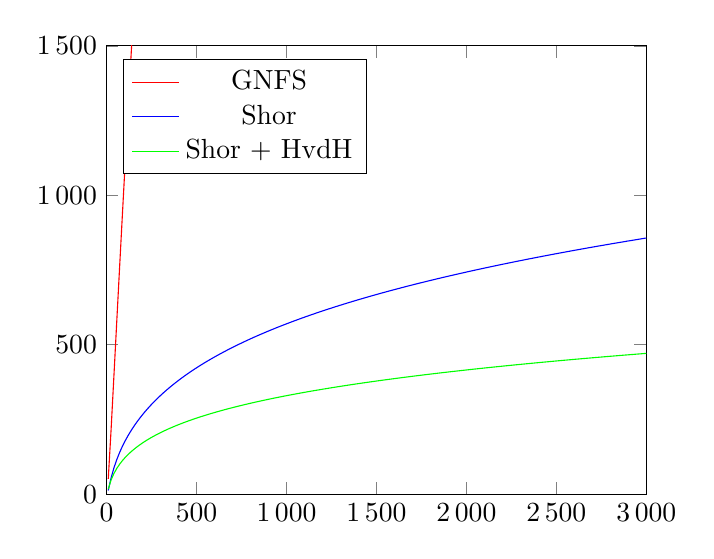
\begin{tikzpicture}
    \begin{axis}[
        xmin=0,
        xmax=3000,
        ymin=0,
        ymax=1500,
        domain=-100:3000,
        samples=200,
        legend pos=north west
    ]
        \addplot[color=red]{exp(1.9 * log2(x)^(1/3) * log2(log2(x))^(2/3) )};
        \addplot[color=blue]{(log2(x)^2)*log2(log2(x))*log2(log2(log2(x)))};
        \addplot[color=green]{(log2(x)^2)*log2(log2(x))};

        \legend{GNFS,Shor, Shor + HvdH};
    \end{axis}
    \end{tikzpicture}
}
\captionof{figure}{
    A comparison of integer factoring algorithms
}
\label{fig:integerFactoringComparison}

\

\subsection{Alternative Visualisation for Tensor Product}
\label{appendix:AlternativeVisualTensorProduct}

A tensor product of two matrices can (informally) also be visualised as the following,
where the ``nested'' matrices are expanded at the end
(the brackets are removed) into one big resultant matrix:

\begin{equation*}
\begin{split}
\begin{bmatrix}
\textcolor{LimeGreen}{1} & \textcolor{orange}{2} \\
\textcolor{PineGreen}{3} & \textcolor{Red}{4}
\end{bmatrix}
\otimes
\begin{bmatrix}
5 & 6 \\
7 & 8
\end{bmatrix}
& =
\begin{bmatrix}
\textcolor{LimeGreen}{1}\begin{bmatrix}
5 & 6 \\
7 & 8
\end{bmatrix} & \textcolor{orange}{2}\begin{bmatrix}
5 & 6 \\
7 & 8
\end{bmatrix} \\
\textcolor{PineGreen}{3}\begin{bmatrix}
5 & 6 \\
7 & 8
\end{bmatrix} & \textcolor{Red}{4}\begin{bmatrix}
5 & 6 \\
7 & 8
\end{bmatrix} \\
\end{bmatrix} \\
& =
\begin{bmatrix}
\begin{bmatrix}
\textcolor{LimeGreen}{1}(5) & \textcolor{LimeGreen}{1}(6) \\
\textcolor{LimeGreen}{1}(7) & \textcolor{LimeGreen}{1}(8)
\end{bmatrix} & \begin{bmatrix}
\textcolor{orange}{2}(5) & \textcolor{orange}{2}(6) \\
\textcolor{orange}{2}(7) & \textcolor{orange}{2}(8)
\end{bmatrix} \\
\begin{bmatrix}
\textcolor{PineGreen}{3}(5) & \textcolor{PineGreen}{3}(6) \\
\textcolor{PineGreen}{3}(7) & \textcolor{PineGreen}{3}(8)
\end{bmatrix} & \begin{bmatrix}
\textcolor{Red}{4}(5) & \textcolor{Red}{4}(6) \\
\textcolor{Red}{4}(7) & \textcolor{Red}{4}(8)
\end{bmatrix} \\
\end{bmatrix} \\
& =
\begin{bmatrix}
\textcolor{LimeGreen}{1}(5) & \textcolor{LimeGreen}{1}(6) & \textcolor{orange}{2}(5) & \textcolor{orange}{2}(6) \\
\textcolor{LimeGreen}{1}(7) & \textcolor{LimeGreen}{1}(8) & \textcolor{orange}{2}(7) & \textcolor{orange}{2}(8) \\
\textcolor{PineGreen}{3}(5) & \textcolor{PineGreen}{3}(6) & \textcolor{Red}{4}(5) & \textcolor{Red}{4}(6) \\
\textcolor{PineGreen}{3}(7) & \textcolor{PineGreen}{3}(8) & \textcolor{Red}{4}(7) & \textcolor{Red}{4}(8)
\end{bmatrix}
\end{split}
\end{equation*}

This is not a formal definition but merely a visualisation strategy,
as nested matrices can have a different and concrete meaning in mathematics. \\

Certainly thinking about this example from a high-level-programming-language point of view,
there would be a difference between a 2-level nested list/array such as this in python:

\begin{verbatim}
list1 = [
    [1*5, 1*6, 2*6, 2*6],
    [1*7, 1*8, 2*7, 2*8],
    [3*5, 3*6, 4*5, 4*6],
    [3*7, 3*8, 4*7, 4*8]
]

\end{verbatim}

And a more convoluted 4-level nested list:

\begin{verbatim}
list2 = [
    [
        [[1*5, 1*6], [1*7, 1*8]],
        [[2*5, 2*6], [2*7, 2*8]]
    ],
    [
        [[3*5, 3*6], [3*7, 3*8]],
        [[4*5, 4*6], [4*7, 4*8]]
    ],
]
\end{verbatim}

Even if physically, especially in a lower-level language such as C, such datastructures
would end up being stored in memory as a single continuous ``array'' (chunk) of 32 or 64-bit integers. \\

\subsection{Bloch Sphere Parameters Solution for the Basis State $\ket{1}$}
\label{appendix:BlochSphereSolutionExample}

This section provides a written out solution to computing the Bloch Sphere parameters
$0\le \theta \le \pi$ and $0 \le \varphi < 2 \pi$ (both radians),
 for visualusing the one-qubit basis state $\ket{1}$. $\ket{0}$ does not need to be computed as it has $\theta=0, \varphi=0$.
Other pure states (superpositons) are computed analogously to the following.

We start by writing down the state vector in terms of (Equation \ref{eq:purestate1}) and equating it to (Equation \ref{eq:purestate2}).
For the pure states this is obviously quite simple, $\ket{1}$ having $\alpha=0, \beta=1$ (and $\ket{0}$ having $\alpha=1, \beta=0$).

Solving this for $\ket{1}$:
\begin{multline*}
    \ket{1} = \cos{(\theta/2)}\ket{0} + e^{i\varphi}\sin{(\theta/2)}\ket{1} \\
\begin{split}
\Leftrightarrow
\begin{bmatrix}
    0 \\
    1
\end{bmatrix}
=
\begin{bmatrix}
    \cos{(\theta/2)} \\
    e^{i\varphi}\sin{(\theta/2)}
\end{bmatrix}
& \Leftrightarrow
\setlength\arraycolsep{1pt}
\left\{
\begin{array}{rcrcrc@{\qquad}l}
\cos{(\theta/2)}   &   =  0\\
e^{i\varphi}\sin{(\theta/2)}  &   =  1\\
\end{array}
\right.
\\
\end{split}
\end{multline*}

We solve for $\theta$:
\begin{multline*}
\begin{split}
 \ \ &
\begin{array}{rcrcrc@{\qquad}l}
\cos{^{-1}(0)}   &  = \theta/2\\
\end{array}
\\
& \Leftrightarrow
\begin{array}{rcrcrc@{\qquad}l}
2\cos{^{-1}(0)}   &  = \theta\\
\end{array}
\\
& \Leftrightarrow
\begin{array}{rcrcrc@{\qquad}l}
2(\frac{\pi}{2})   &  = \theta\\
\end{array}
\text{ \ \ \ \ [since } 0\le \theta \le \pi \text{]}
\\
& \Leftrightarrow
\begin{array}{rcrcrc@{\qquad}l}
\pi  &  = \theta\\
\end{array}
\end{split}
\end{multline*}

We next solve for $\varphi$ using $\theta$:
\begin{multline*}
\begin{split}
\ \ &
\begin{array}{rcrcrc@{\qquad}l}
e^{i\varphi}\sin{(\pi/2)}  &   =  1\\
\end{array}
\text{ [fill in } \theta=\pi \text{]}
\\
& \Leftrightarrow
\begin{array}{rcrcrc@{\qquad}l}
e^{i\varphi}(1)  &   =  1\\
\end{array}
\\
& \Leftrightarrow
\begin{array}{rcrcrc@{\qquad}l}
\ln{(e^{i\varphi})}  &   =  \ln{(1)}\\
\end{array}
\\
& \Leftrightarrow
\begin{array}{rcrcrc@{\qquad}l}
i\varphi  &   =  0\\
\end{array}
\\
& \Leftrightarrow
\begin{array}{rcrcrc@{\qquad}l}
\varphi  &   =  0/i\\
\end{array}
\\
& \Leftrightarrow
\begin{array}{rcrcrc@{\qquad}l}
\varphi  &   =  0\\
\end{array}
\end{split}
\end{multline*}

This solution, $\theta = \pi, \varphi=0$, in turn gives a vector pointing straight down on the Bloch Sphere (Figure \ref{fig:blochsphere}) to represent $\ket{1}$.

\subsection{Basic Gate Library}
\label{appendix:BasicGateLibrary}

The ``Basic Gate Library'' of all quantum logic gates included in our application is given in Table \ref{table:gatelib}.

\begin{table}[!h]
\begin{center}
    \caption{Basic Gate Library}
    \label{table:gatelib}
\begin{tabular}{ccc}
    \toprule
    gate & name (alternative names) & matrix \\
    \midrule
    % \textcolor{black}{\rule[3pt]{2mm}{0.2mm}}\vspace{-\baselineskip}\par\noindent
    % \fboxsep=3mm \fboxrule=0mm
    % \fcolorbox{black}{OrangeRed!60!BrickRed!100}{H}\vspace{-\baselineskip}\par\noindent
    % \textcolor{black}{\rule[3pt]{2mm}{0.2mm}}\vspace{-\baselineskip}\par\noindent

    \begin{minipage}[c]{1cm}
        \includegraphics{img/gate_h.png}
    \end{minipage}

    & H (Hadamard)
    &
    $
    \frac{1}{\sqrt{2}}
    \begin{bmatrix}
        1 & 1 \\
        1 & -1
    \end{bmatrix}
    $
    \\
    \begin{minipage}[c]{1cm}
        \includegraphics{img/gate_x.png}
    \end{minipage}
    & X (Pauli-X, NOT)
    &
    $
    \begin{bmatrix}
        0 & 1 \\
        1 & 0
    \end{bmatrix}
    $
    \\
    \begin{minipage}[c]{1cm}
        \includegraphics{img/gate_cnot.png}
    \end{minipage}
    & CNOT (Controlled NOT)
    &
    $
    \begin{bmatrix}
        1 & 0 & 0 & 0 \\
        0 & 1 & 0 & 0 \\
        0 & 0 & 0 & 1 \\
        0 & 0 & 1 & 0
    \end{bmatrix}
    $
    \\
    \begin{minipage}[c]{1cm}
        \includegraphics{img/gate_swap.png}
    \end{minipage}
    & SWAP
    &
    $
    \begin{bmatrix}
        1 & 0 & 0 & 0 \\
        0 & 0 & 1 & 0 \\
        0 & 1 & 0 & 0 \\
        0 & 0 & 0 & 1
    \end{bmatrix}
    $
    \\
    \begin{minipage}[c]{1cm}
        \includegraphics{img/gate_y.png}
    \end{minipage}
    & Y (Pauli-Y)
    &
    $
    \begin{bmatrix}
        0 & -i \\
        i & 0
    \end{bmatrix}
    $
    \\
    \begin{minipage}[c]{1cm}
        \includegraphics{img/gate_z.png}
    \end{minipage}
    & Z (Pauli-Z)
    &
    $
    \begin{bmatrix}
        1 & 0 \\
        0 & -1
    \end{bmatrix}
    $
    \\
    \begin{minipage}[c]{1cm}
        \includegraphics{img/gate_cz.png}
    \end{minipage}
    & CZ (Controlled Z)
    &
    $
    \begin{bmatrix}
        1 & 0 & 0 & 0 \\
        0 & 1 & 0 & 0 \\
        0 & 0 & 1 & 0 \\
        0 & 0 & 0 & -1
    \end{bmatrix}
    $
    \\
    \begin{minipage}[c]{1cm}
        \includegraphics{img/gate_s.png}
    \end{minipage}
    & S (Phase, P)
    &
    $
    \begin{bmatrix}
        1 & 0 \\
        0 & i
    \end{bmatrix}
    $
    \\
    \begin{minipage}[c]{1cm}
        \includegraphics{img/gate_cs.png}
    \end{minipage}
    & Controlled S (Phase, P)
    &
    $
    \begin{bmatrix}
        1 & 0 & 0 & 0 \\
        0 & 1 & 0 & 0 \\
        0 & 0 & 1 & 0 \\
        0 & 0 & 0 & i
    \end{bmatrix}
    $
    \\
    \begin{minipage}[c]{1cm}
        \includegraphics{img/gate_t.png}
    \end{minipage}
    & T ($\pi/8$)
    &
    $
    \begin{bmatrix}
        1 & 0 \\
        0 & e^{i\pi/4}
    \end{bmatrix}
    $
    \\
    \begin{minipage}[c]{1cm}
        \includegraphics{img/gate_t_dagger.png}
    \end{minipage}
    & T$^\dagger$ (T$^*$)
    &
    $
    \begin{bmatrix}
        1 & 0 \\
        0 & e^{-i\pi/4}
    \end{bmatrix}
    $
    \\
    \begin{minipage}[c]{1cm}
        \includegraphics{img/gate_measure.png}
    \end{minipage}
    & Measure
    &
    -
    \\
    \bottomrule
\end{tabular}
\end{center}
\end{table}

\subsection{Graph Data Structure Example Table}
\label{appendix:GraphDataStructureExampleTable}

The two main methods for storing the widely-known "graph" data structure (directed or undirected) in memory are:
(1) the adjacency matrix; and (2) adjacency list. This section provides an example of an adjacency matrix representation of a graph.
Of interest is the \textit{concept} of ``mapping'' items in a ``from-to'' relationship using a matrix.

Given the following directed graph:\\

\centerline{
    \includegraphics[width=0.25\textwidth]{img/basic_graph.png}
}
\captionof{figure}{
    A basic directed graph consisting of 3 nodes: 0, 1, and 2
}
\label{fig:basicGraphExample}
 \

This graph can be represented by the following adjacency matrix:

\begin{center}
\begin{tabular}{|c|c|c|c|}
    \hline
    \ & \textbf{0} & \textbf{1} & \textbf{2} \\
    \hline
    \textbf{0} & 0 & 0 & 1 \\
    \textbf{1} & 1 & 0 & 0 \\
    \textbf{2} & 0 & 0 & 1 \\
    \hline
\end{tabular}
\end{center}

As is surely widely understood, cells with ``0'' represent the absence of a direct edge/link between the node in the row/column, and a ``1''
represents the presence of such a link. In this example it was chosen to have the ``rows'' represent the ``from''
and the ``columns'' represent the ``to'' of an edge/link.

\subsection{Algorithmic Method for Controlled Gate Construction: Example}
\label{appendix:AlgoMethodControlledGateExample}

This section provides an example of how one can construct a Controlled NOT matrix
for a system of three qubits, as shown in (Figure \ref{fig:examplethreequbitscontrolledgateconstruction}),
using qubit $1$ ($q_1$) as the \textit{control-qubit} (middle line), and qubit $2$ ($q_2$) (bottom line) as the
\textit{target-qubit}. Qubit $0$ ($q_0$) (top line) will remain unaffected by this matrix.
\newline

\textbf{``If qubit $j=1$ is $\ket{0}$, then do nothing to qubit $k=2$'':}
\begin{multline*}
    M_{q_{j}=\ket{0}}
    = I \otimes \underbrace{\ket{0} \bra{0}}_{j=1} \otimes \underbrace{I}_{k=2}
    =
    \begin{bmatrix}
        1 & 0 \\
        0 & 1
    \end{bmatrix}
    \otimes
    \begin{bmatrix}
        1 & 0 \\
        0 & 0
    \end{bmatrix}
    \otimes
    \begin{bmatrix}
        1 & 0 \\
        0 & 1
    \end{bmatrix} \\
    =
    \begin{bmatrix}
        1 & 0 & 0 & 0 \\
        0 & 0 & 0 & 0 \\
        0 & 0 & 1 & 0 \\
        0 & 0 & 0 & 0
    \end{bmatrix}
    \otimes
    \begin{bmatrix}
        1 & 0 \\
        0 & 1
    \end{bmatrix}
    =
    \begin{bmatrix}
        1 & 0 & 0 & 0 & 0 & 0 & 0 & 0 \\
        0 & 1 & 0 & 0 & 0 & 0 & 0 & 0 \\
        0 & 0 & 0 & 0 & 0 & 0 & 0 & 0 \\
        0 & 0 & 0 & 0 & 0 & 0 & 0 & 0 \\
        0 & 0 & 0 & 0 & 1 & 0 & 0 & 0 \\
        0 & 0 & 0 & 0 & 0 & 1 & 0 & 0 \\
        0 & 0 & 0 & 0 & 0 & 0 & 0 & 0 \\
        0 & 0 & 0 & 0 & 0 & 0 & 0 & 0 \\
    \end{bmatrix}
\end{multline*}

\textbf{``If qubit $j=1$ is $\ket{1}$, then apply gate X to qubit $k=2$'':}
\begin{multline*}
    M_{q_{j}=\ket{1}}
    = I \otimes \underbrace{\ket{1} \bra{1}}_{j=1} \otimes \underbrace{X}_{k=2}
    =
    \begin{bmatrix}
        1 & 0 \\
        0 & 1
    \end{bmatrix}
    \otimes
    \begin{bmatrix}
        0 & 0 \\
        0 & 1
    \end{bmatrix}
    \otimes
    \begin{bmatrix}
        0 & 1 \\
        1 & 0
    \end{bmatrix} \\
    =
    \begin{bmatrix}
        0 & 0 & 0 & 0 \\
        0 & 1 & 0 & 0 \\
        0 & 0 & 0 & 0 \\
        0 & 0 & 0 & 1
    \end{bmatrix}
    \otimes
    \begin{bmatrix}
        0 & 1 \\
        1 & 0
    \end{bmatrix}
    =
    \begin{bmatrix}
        0 & 0 & 0 & 0 & 0 & 0 & 0 & 0 \\
        0 & 0 & 0 & 0 & 0 & 0 & 0 & 0 \\
        0 & 0 & 0 & 1 & 0 & 0 & 0 & 0 \\
        0 & 0 & 1 & 0 & 0 & 0 & 0 & 0 \\
        0 & 0 & 0 & 0 & 0 & 0 & 0 & 0 \\
        0 & 0 & 0 & 0 & 0 & 0 & 0 & 0 \\
        0 & 0 & 0 & 0 & 0 & 0 & 0 & 1 \\
        0 & 0 & 0 & 0 & 0 & 0 & 1 & 0 \\
    \end{bmatrix}
\end{multline*}

\textbf{Resulting unitary transformation matrix (``system-level operation matrix''):}
\begin{multline*}
    CNOT_{j,k} = M_{q_{j}=\ket{0}} + M_{q_{j}=\ket{1}}
    = \\
    \begin{bmatrix}
        1 & 0 & 0 & 0 & 0 & 0 & 0 & 0 \\
        0 & 1 & 0 & 0 & 0 & 0 & 0 & 0 \\
        0 & 0 & 0 & 0 & 0 & 0 & 0 & 0 \\
        0 & 0 & 0 & 0 & 0 & 0 & 0 & 0 \\
        0 & 0 & 0 & 0 & 1 & 0 & 0 & 0 \\
        0 & 0 & 0 & 0 & 0 & 1 & 0 & 0 \\
        0 & 0 & 0 & 0 & 0 & 0 & 0 & 0 \\
        0 & 0 & 0 & 0 & 0 & 0 & 0 & 0 \\
    \end{bmatrix}
    +
    \begin{bmatrix}
        0 & 0 & 0 & 0 & 0 & 0 & 0 & 0 \\
        0 & 0 & 0 & 0 & 0 & 0 & 0 & 0 \\
        0 & 0 & 0 & 1 & 0 & 0 & 0 & 0 \\
        0 & 0 & 1 & 0 & 0 & 0 & 0 & 0 \\
        0 & 0 & 0 & 0 & 0 & 0 & 0 & 0 \\
        0 & 0 & 0 & 0 & 0 & 0 & 0 & 0 \\
        0 & 0 & 0 & 0 & 0 & 0 & 0 & 1 \\
        0 & 0 & 0 & 0 & 0 & 0 & 1 & 0 \\
    \end{bmatrix} \\
    =
    \begin{matrix}
        \ \ {\scriptscriptstyle 000}
        \ \ {\scriptscriptstyle 001}
        \ {\scriptscriptstyle 0\textcolor{blue}{1}\textcolor{red}{0}}
        \ \ {\scriptscriptstyle 0\textcolor{blue}{1}\textcolor{red}{1}}
        \ {\scriptscriptstyle 100}
        \ \ {\scriptscriptstyle 101}
        \ {\scriptscriptstyle 1\textcolor{blue}{1}\textcolor{red}{0}}
        \ \ {\scriptscriptstyle 1\textcolor{blue}{1}\textcolor{red}{1}}
        \\
        \begin{matrix}
            {\scriptscriptstyle 000} \\
            {\scriptscriptstyle 001} \\
            {\scriptscriptstyle 0\textcolor{blue}{1}\textcolor{red}{0}} \\
            {\scriptscriptstyle 0\textcolor{blue}{1}\textcolor{red}{1}} \\
            {\scriptscriptstyle 100} \\
            {\scriptscriptstyle 101} \\
            {\scriptscriptstyle 1\textcolor{blue}{1}\textcolor{red}{0}} \\
            {\scriptscriptstyle 1\textcolor{blue}{1}\textcolor{red}{1}}
        \end{matrix}
        \begin{bmatrix}
            1 & 0 & 0 & 0 & 0 & 0 & 0 & 0 \\
            0 & 1 & 0 & 0 & 0 & 0 & 0 & 0 \\
            0 & 0 & 0 & 1 & 0 & 0 & 0 & 0 \\
            0 & 0 & 1 & 0 & 0 & 0 & 0 & 0 \\
            0 & 0 & 0 & 0 & 1 & 0 & 0 & 0 \\
            0 & 0 & 0 & 0 & 0 & 1 & 0 & 0 \\
            0 & 0 & 0 & 0 & 0 & 0 & 0 & 1 \\
            0 & 0 & 0 & 0 & 0 & 0 & 1 & 0 \\
        \end{bmatrix}
    \end{matrix}
\end{multline*}

\begin{figure}[tbp]
    \centerline{
        \includegraphics[width=0.5\textwidth]{img/three-qubit-bell-matrix-construction-example.png}
    }
    \caption{Three qubit circuit with H targetting qubit 1 followed by Controlled NOT targetting qubit 2, using qubit 1 as control}
    \label{fig:examplethreequbitscontrolledgateconstruction}
\end{figure}

All the $2^3=8$ mappings are given below, with the non-identity mappings highlighted
(\textcolor{blue}{control} bit \textcolor{blue}{blue}, \textcolor{red}{target} bit \textcolor{red}{red}):
\begin{gather*}
    \text{\textbf{input}} \xrightarrow{\text{CNOT}} \text{\textbf{output}} \\
    \ket{000} \longrightarrow \ket{000} \\
    \ket{001} \longrightarrow \ket{001} \\
    \ket{0\textcolor{blue}{1}\textcolor{red}{0}} \longrightarrow \ket{0\textcolor{blue}{1}\textcolor{red}{1}} \\
    \ket{0\textcolor{blue}{1}\textcolor{red}{1}} \longrightarrow \ket{0\textcolor{blue}{1}\textcolor{red}{0}} \\
    \ket{100} \longrightarrow \ket{100} \\
    \ket{101} \longrightarrow \ket{101} \\
    \ket{1\textcolor{blue}{1}\textcolor{red}{0}} \longrightarrow \ket{1\textcolor{blue}{1}\textcolor{red}{1}} \\
    \ket{1\textcolor{blue}{1}\textcolor{red}{1}} \longrightarrow \ket{1\textcolor{blue}{1}\textcolor{red}{0}} \\
\end{gather*}
To fully explain (Figure \ref{fig:examplethreequbitscontrolledgateconstruction}),
we can observe that the initial state of the qubit system is $\ket{0\textcolor{blue}{0}\textcolor{red}{0}}$.
Next, a H (Hadamard) gate is applied to the middle qubit — \textcolor{blue}{qubit $1$}, highlighted blue —
making a superposition with two possible states with equal probability: one where \textcolor{blue}{qubit $1$} is $\ket{0}$
and one where \textcolor{blue}{qubit $1$} is $\ket{1}$. Qubit $0$ (top most in the circuit, also
left-most in the input state vector and in the binary string) is always $\ket{0}$. \\

If \textcolor{blue}{qubit $1$} is $\ket{1}$, we invert \textcolor{red}{qubit $2$} to be $\ket{1}$,
which is $\ket{0}$ initially
(highlighted red in the input vector). If \textcolor{blue}{qubit $1$} is $\ket{0}$,
we don't do anything with \textcolor{red}{qubit $2$} and it stays $\ket{0}$. \\

The only possible output states in this case are: \\
(1) $\boldsymbol{\ket{0\textcolor{blue}{0}\textcolor{red}{0}}}$ (\textcolor{blue}{$q_{1}$} not flipped,
hence CNOT no effect on \textcolor{red}{$q_{2}$}); and \\
(2) $\boldsymbol{\ket{0\textcolor{blue}{1}\textcolor{red}{1}}}$ (\textcolor{blue}{$q_{1}$} was flipped,
hence CNOT also flipped \textcolor{red}{$q_{2}$} conditionally).

With equal probability $p=0.5$ each. \\

\subsection{Bell States}
\label{appendix:BellStates}

\begin{center}
\begin{tabular}{cc}
    \toprule
    Bell State & Formula \\
    \midrule
    $\ket{\boldsymbol{\upphi}^+}$ & $\frac{\ket{00} + \ket{11}}{\sqrt{2}}$ \\
    $\ket{\boldsymbol{\upphi}^-}$ & $\frac{\ket{00} - \ket{11}}{\sqrt{2}}$ \\
    $\ket{\boldsymbol{\uppsi}^+}$ & $\frac{\ket{01} + \ket{10}}{\sqrt{2}}$ \\
    $\ket{\boldsymbol{\uppsi}^-}$ & $\frac{\ket{01} - \ket{10}}{\sqrt{2}}$ \\
    \bottomrule
\end{tabular}
\end{center}
 \


\subsection{Classical Logic Circuits Reference}
\label{appendix:ClassicalLogicGates}

This section provides an overview of the standard classical logic gates and their truth tables.
This section may be of interest when comparing to the corresponding quantum implementations of these basic operations. \\

\textbf{Classical NOT}

\centerline{
    \includegraphics[width=0.225\textwidth]{img/classical-not-gate.png}
}
\captionof{figure}{
    A classical logic circuit NOT gate
}
\label{fig:classicalNot}

\begin{center}
\begin{tabular}{|c|c|}
    \hline
    $A$ & $\neg A$ \\
    \hline
    0 & 1 \\
    1 & 0 \\
    \hline
\end{tabular}
\end{center}


\textbf{Classical AND}


\centerline{
    \includegraphics[width=0.225\textwidth]{img/classical-and-gate.png}
}
\captionof{figure}{
    A classical logic circuit AND gate
}
\label{fig:classicalAnd}

\begin{center}
\begin{tabular}{|c|c|c|}
    \hline
    $A$ & $B$ & $A \land B$ \\
    \hline
    0 & 0 & 0 \\
    0 & 1 & 0 \\
    1 & 0 & 0 \\
    1 & 1 & 1 \\
    \hline
\end{tabular}
\end{center}


\textbf{Classical OR}


\centerline{
    \includegraphics[width=0.225\textwidth]{img/classical-or-gate.png}
}
\captionof{figure}{
    A classical logic circuit OR gate
}
\label{fig:classicalOr}

\begin{center}
\begin{tabular}{|c|c|c|}
    \hline
    $A$ & $B$ & $A \lor B$ \\
    \hline
    0 & 0 & 0 \\
    0 & 1 & 1 \\
    1 & 0 & 1 \\
    1 & 1 & 1 \\
    \hline
\end{tabular}
\end{center} \ \\


\textbf{XOR implemented by composing basic classical logic gates} \ \\

\centerline{
    \includegraphics[width=0.5\textwidth]{img/XOR_gate_based_on_2-2_AOI_gate.svg.png}
}
\captionof{figure}{
    `XOR' implemented using a combination of classical logic gates\cite{ref:img:OAIGateClassical}
}
\label{fig:logicalXORcircuit}

\subsection{Quantum Circuit Examples}
\label{appendix:QuantumCircuitExamples}

This section provides more quantum circuit examples that were left out of the main text for the sake of brevity.


\centerline{
    \includegraphics[width=0.225\textwidth]{img/x-circuit.png}
}
\captionof{figure}{
    A single-qubit, single-X-gate quantum circuit
}
\label{fig:singlequbitsinglegatecirquit}


\centerline{
    \includegraphics[width=0.225\textwidth]{img/single-gate-2-qubits-alt.png}
}
\captionof{figure}{
    A circuit that is equivalent to (Figure \ref{fig:twoqubittwosinglegateresult})
}
\label{fig:singlequbittwogatecirquit_alt}

\centerline{
    \includegraphics[width=0.5\textwidth]{img/multi-gate-bell-state-result.png}
}
\captionof{figure}{
    A circuit composed of a Hadamard and Controlled NOT gate, producing output state $\ket{\boldsymbol{\upphi}^+}$ — one of the \textit{Bell States}
}
\label{fig:controlledgate2qubitresult}

\centerline{
    \includegraphics[width=0.5\textwidth]{img/repeated_swapping_to_do_cnot_last_bits.png}
}
\captionof{figure}{
    One approach to interpret applying an operation to two qubits that are not situated on the first two lines
}
\label{fig:repeatedSwappingToDoCnotOnLastBits}


\centerline{
    \includegraphics[width=0.5\textwidth]{img/circuit_and_v2.png}
}
\captionof{figure}{
    An alternative way to implement a Toffoli gate, equivalent to (Figure \ref{fig:circuitAndV1})\cite{ref:quantumvialinearalgebra}
}
\label{fig:circuitAndV2}



\centerline{
    \includegraphics[width=0.5\textwidth]{img/deutsch_circuit_result_constant_0.png}
}
\captionof{figure}{
    The circuit for the Deutsch algorithm with $U_f$ using $f(x)=0$
}
\label{fig:deutschCircuitConstant0}


\centerline{
    \includegraphics[width=0.5\textwidth]{img/deutsch_circuit_result_constant_1.png}
}
\captionof{figure}{
    The circuit for the Deutsch algorithm with $U_f$ using $f(x)=1$
}
\label{fig:deutschCircuitConstant1}


\centerline{
    \includegraphics[width=0.5\textwidth]{img/deutsch_circuit_result_fx_x.png}
}
\captionof{figure}{
    The circuit for the Deutsch algorithm with $U_f$ using $f(x)=x$
}
\label{fig:deutschCircuitFxIsx}


\centerline{
    \includegraphics[width=0.5\textwidth]{img/deutsch_circuit_result_fx_not_x.png}
}
\captionof{figure}{
    The circuit for the Deutsch algorithm with $U_f$ using $f(x)=\lnot x$
}
\label{fig:deutschCircuitFxIsNotx}

 \

\subsection{Deutsch Algorithm $U_{f}$ Matrices}
\label{appendix:deutschAlgorithmMatrices}

This section covers all 4 possible unitary transformation matrices that may be used as the \textit{oracle} $U_{f}$
in the Deutsch algorithm (Deutsch-Josza with $n=1$).
We note again that we are looking to determine a matrix representation for the following equation:

\begin{equation*}
    \ket{x, y} \xrightarrow{U_f} \ket{x, y \oplus f(x)}
\end{equation*}

In total we have 4 functions that can be distinguished as operating on $1$ input bit:
\begin{itemize}
 \item \textit{Constant} functions: $f(x) = 0$ and $f(x) = 1$
 \item \textit{Balanced} functions: $f(x) = x$ and $f(x) = \lnot x$
\end{itemize}
 \ \\

\textbf{Balanced function $f(x) = x$:} \\

For this function we can determine the truth table:

\begin{center}
\begin{tabular}{|c|c|c|c|}
    \hline
    $x$ & $y$ & $f(x) = x$ & $y \oplus f(x)$\\
    \hline
    0 & 0 & 0 & 0 \\
    0 & 1 & 0 & 1 \\
    1 & 0 & 1 & 1 \\
    1 & 1 & 1 & 0 \\
    \hline
\end{tabular}
\end{center}

Hence the state maps for the gate $U_f$ would have to map:

\begin{gather*}
    \ket{0, 0} \xrightarrow{U_f} \ket{0, 0} \\
    \ket{0, 1} \xrightarrow{U_f} \ket{0, 1} \\
    \ket{1, 0} \xrightarrow{U_f} \ket{1, 1} \\
    \ket{1, 1} \xrightarrow{U_f} \ket{1, 0} \\
\end{gather*}

This corresponds to the following matrix, which is in fact the CNOT matrix (see Appendix \ref{appendix:BasicGateLibrary}):

\begin{center}
$
\begin{matrix}
    \ \ \ {\scriptstyle 00} \ \ {\scriptstyle 01} \ {\scriptstyle 10} \ \ {\scriptstyle 11} \ \ \ \ \ \ \ \ \ \ \ \ \
    \\
    \begin{matrix}
    {\scriptstyle 00} \\
    {\scriptstyle 01} \\
    {\scriptstyle 10} \\
    {\scriptstyle 11}
    \end{matrix}
    \begin{bmatrix}
    1 & 0 & 0 & 0 \\
    0 & 1 & 0 & 0 \\
    0 & 0 & 0 & 1 \\
    0 & 0 & 1 & 0
    \end{bmatrix}
    \eqcolon \text{\textit{CNOT}}
\end{matrix}
$
\end{center}
 \ \\

\textbf{Balanced function $f(x) = \lnot x$:} \\

Corresponding truth table:

\begin{center}
\begin{tabular}{|c|c|c|c|}
    \hline
    $x$ & $y$ & $f(x) = \lnot x$ & $y \oplus f(x)$\\
    \hline
    0 & 0 & 1 & 1 \\
    0 & 1 & 1 & 0 \\
    1 & 0 & 0 & 0 \\
    1 & 1 & 0 & 1 \\
    \hline
\end{tabular}
\end{center}

Mappings for corresponding $U_f$:

\begin{gather*}
    \ket{0, 0} \xrightarrow{U_f} \ket{0, 1} \\
    \ket{0, 1} \xrightarrow{U_f} \ket{0, 0} \\
    \ket{1, 0} \xrightarrow{U_f} \ket{1, 0} \\
    \ket{1, 1} \xrightarrow{U_f} \ket{1, 1} \\
\end{gather*}

This corresponds to the following matrix:

\begin{center}
$
\begin{matrix}
    \ \ \ {\scriptstyle 00} \ \ {\scriptstyle 01} \ {\scriptstyle 10} \ \ {\scriptstyle 11}
    \\
    \begin{matrix}
    {\scriptstyle 00} \\
    {\scriptstyle 01} \\
    {\scriptstyle 10} \\
    {\scriptstyle 11}
    \end{matrix}
    \begin{bmatrix}
    0 & 1 & 0 & 0 \\
    1 & 0 & 0 & 0 \\
    0 & 0 & 1 & 0 \\
    0 & 0 & 0 & 1
    \end{bmatrix}
\end{matrix}
$
\end{center}

Note that this matrix inverses the behaviour for CNOT in a certain sense.
For this matrix we flip the second qubit if the first qubit is not set.

This can be simulated by the following gates:

\centerline{
    \includegraphics[width=0.225\textwidth]{img/oracle_f_for_not_x.png}
}

Here, we first flip $\ket{x}$, then apply CNOT based on this flipped value, and reset the flip once that is done.

Alternatively, $U_f$ is given by:
\begin{multline*}
(X \otimes I)(CNOT)(X \otimes I) \\
=
\left(
\begin{bmatrix}
    0 & 1 \\
    1 & 0 \\
\end{bmatrix}
\otimes
\begin{bmatrix}
    1 & 0 \\
    0 & 1 \\
\end{bmatrix}
\right)
\begin{bmatrix}
    1 & 0 & 0 & 0 \\
    0 & 1 & 0 & 0 \\
    0 & 0 & 0 & 1 \\
    0 & 0 & 1 & 0
\end{bmatrix}
\left(
\begin{bmatrix}
    0 & 1 \\
    1 & 0 \\
\end{bmatrix}
\otimes
\begin{bmatrix}
    1 & 0 \\
    0 & 1 \\
\end{bmatrix}
\right) \\
=
\begin{bmatrix}
    0 & 0 & 1 & 0\\
    0 & 0 & 0 & 1\\
    1 & 0 & 0 & 0\\
    0 & 1 & 0 & 0\\
\end{bmatrix}
\begin{bmatrix}
    1 & 0 & 0 & 0 \\
    0 & 1 & 0 & 0 \\
    0 & 0 & 0 & 1 \\
    0 & 0 & 1 & 0
\end{bmatrix}
\begin{bmatrix}
    0 & 0 & 1 & 0\\
    0 & 0 & 0 & 1\\
    1 & 0 & 0 & 0\\
    0 & 1 & 0 & 0\\
\end{bmatrix} \\
=
\begin{bmatrix}
    0 & 1 & 0 & 0 \\
    1 & 0 & 0 & 0 \\
    0 & 0 & 1 & 0 \\
    0 & 0 & 0 & 1
\end{bmatrix}
\end{multline*}

\textbf{Constant function $f(x) = 0$:} \\

For this function we can determine the truth table:

\begin{center}
\begin{tabular}{|c|c|c|c|}
    \hline
    $x$ & $y$ & $f(x) = 0$ & $y \oplus f(x)$\\
    \hline
    0 & 0 & 0 & 0 \\
    0 & 1 & 0 & 1 \\
    1 & 0 & 0 & 0 \\
    1 & 1 & 0 & 1 \\
    \hline
\end{tabular}
\end{center}

Mappings for corresponding $U_f$:

\begin{gather*}
    \ket{0, 0} \xrightarrow{U_f} \ket{0, 0} \\
    \ket{0, 1} \xrightarrow{U_f} \ket{0, 1} \\
    \ket{1, 0} \xrightarrow{U_f} \ket{1, 0} \\
    \ket{1, 1} \xrightarrow{U_f} \ket{1, 1} \\
\end{gather*}

We note that $y$ will be unchanged. This is the $4 \times 4$ identity matrix:

\begin{center}
$
\begin{matrix}
    \ \ \ {\scriptstyle 00} \ \ {\scriptstyle 01} \ {\scriptstyle 10} \ \ {\scriptstyle 11}
    \\
    \begin{matrix}
    {\scriptstyle 00} \\
    {\scriptstyle 01} \\
    {\scriptstyle 10} \\
    {\scriptstyle 11}
    \end{matrix}
    \begin{bmatrix}
    1 & 0 & 0 & 0 \\
    0 & 1 & 0 & 0 \\
    0 & 0 & 1 & 0 \\
    0 & 0 & 0 & 1
    \end{bmatrix}
\end{matrix}
$
\end{center}

Hence in this case $U_f$ has no effect. This corresponds to not using any gates/no change.
 \ \\


\textbf{Constant function $f(x) = 1$:} \\

For this function we can determine the truth table:

\begin{center}
\begin{tabular}{|c|c|c|c|}
    \hline
    $x$ & $y$ & $f(x) = 1$ & $y \oplus f(x)$\\
    \hline
    0 & 0 & 1 & 1 \\
    0 & 1 & 1 & 0 \\
    1 & 0 & 1 & 1 \\
    1 & 1 & 1 & 0 \\
    \hline
\end{tabular}
\end{center}

Mappings for corresponding $U_f$:

\begin{gather*}
    \ket{0, 0} \xrightarrow{U_f} \ket{0, 1} \\
    \ket{0, 1} \xrightarrow{U_f} \ket{0, 0} \\
    \ket{1, 0} \xrightarrow{U_f} \ket{1, 1} \\
    \ket{1, 1} \xrightarrow{U_f} \ket{1, 0} \\
\end{gather*}

We note that $y$ is always getting inverted by $U_f$. This is the same as applying an ``unconditional CNOT''
aka simply the X-gate to qubit $y$:

\centerline{
    \includegraphics[width=0.125\textwidth]{img/oracle_f_x_on_y.png}
}

Corresponding to matrix:

\begin{center}
$
(I \otimes X) =
\begin{matrix}
    \ \ \ {\scriptstyle 00} \ \ {\scriptstyle 01} \ {\scriptstyle 10} \ \ {\scriptstyle 11}
    \\
    \begin{matrix}
    {\scriptstyle 00} \\
    {\scriptstyle 01} \\
    {\scriptstyle 10} \\
    {\scriptstyle 11}
    \end{matrix}
    \begin{bmatrix}
    0 & 1 & 0 & 0 \\
    1 & 0 & 0 & 0 \\
    0 & 0 & 0 & 1 \\
    0 & 0 & 1 & 0
    \end{bmatrix}
\end{matrix}
$
\end{center}
 \ \\


\textbf{Computing two H-gates being applied to $\ket{01}$}

We compute (annotated with state-vector indices):
\begin{multline*}
(H \otimes H) \ket{01} \\
=
\left(
\frac{1}{\sqrt{2}}
\begin{bmatrix}
    1 & 1 \\
    1 & -1 \\
\end{bmatrix}
\otimes
\frac{1}{\sqrt{2}}
\begin{bmatrix}
    1 & 1 \\
    1 & -1 \\
\end{bmatrix} \right)
\begin{bmatrix}
    0 \\
    1 \\
    0 \\
    0
\end{bmatrix}
\begin{matrix}
{\scriptstyle 00} \\
{\scriptstyle 01} \\
{\scriptstyle 10} \\
{\scriptstyle 11} \\
\end{matrix} \\
=
\frac{1}{2}
\begin{bmatrix}
    1 & 1 & 1 & 1 \\
    1 & -1 & 1 & -1 \\
    1 & 1 & -1 & -1 \\
    1 & -1 & -1 & 1
\end{bmatrix}
\begin{bmatrix}
    0 \\
    1 \\
    0 \\
    0
\end{bmatrix}
\begin{matrix}
{\scriptstyle 00} \\
{\scriptstyle 01} \\
{\scriptstyle 10} \\
{\scriptstyle 11} \\
\end{matrix} \\
=
\frac{1}{2}
\begin{bmatrix}
    1 \\
    -1 \\
    1 \\
    -1
\end{bmatrix}
\begin{matrix}
{\scriptstyle 00} \\
{\scriptstyle 01} \\
{\scriptstyle 10} \\
{\scriptstyle 11} \\
\end{matrix}
=
\frac{1}{2}(\ket{00} - \ket{01} + \ket{10} - \ket{11})
\tag{A.1}
\label{appendix:eq:twoHGatesDeutsch}
\end{multline*}

This gives us the result of Equation \ref{eq:deutschSuperpositionInitial}.


\subsection{Deutsch's Algorithm: Balanced Functions Proof}
\label{appendix:DeutschsAlgorithmBalancedFunctionsProof}

This solution is based on \cite{ref:SevagGharibianDeutschAlgorithm}.

To prove the expected result for the two \textit{balanced} cases, we note that if $f$ is a \textit{balanced} function,
then $f(0) \ne f(1)$. This also means that $1 \oplus f(0) = f(1)$ and
$1 \oplus f(1) = f(0)$, as we are working with a single bit input and output.
Resuming from Equation \ref{eq:deutschSuperpositionInitial}, we apply either of the two possible $U_f$:
\begin{multline*}
    U_f \frac{1}{2}(\ket{00} - \ket{01} + \ket{10} - \ket{11}) \\
    = \frac{1}{2}(\ket{0, 0 \oplus f(0)} - \ket{0, 1 \oplus f(0)} + \ket{1, 0 \oplus f(1)} - \ket{1, 1 \oplus f(1)}) \\
    = \frac{1}{2}(\ket{0, f(0)} - \ket{0, f(1)} + \ket{1, f(1)} - \ket{1, f(0)}) \\
    = \frac{1}{2}((\ket{0} - \ket{1}) \otimes \ket{f(0)} - (\ket{0} - \ket{1}) \otimes \ket{f(1)}) \\
    = \frac{1}{2}(\ket{0} - \ket{1}) \otimes (\ket{f(0)} - \ket{f(1)}) \\
    = \frac{1}{\sqrt{2}}\ket{-} \otimes (\ket{f(0)} - \ket{f(1)}) \tag{A.2} \label{eq:deutschBalancedEq1}
\end{multline*}

We now know that $q_0$ is in state $\ket{-}$ (which was mentioned in Section \ref{sec:SingleQubitGate}).
If we then rewrite as follows:
\begin{multline*}
    \frac{1}{\sqrt{2}}\ket{-} \otimes (\ket{f(0)} - \ket{f(1)})
    =
    \ket{-} \otimes \frac{1}{\sqrt{2}}(\ket{f(0)} - \ket{f(1)})
\end{multline*}

Then we can observe that: $\frac{1}{\sqrt{2}}(\ket{f(0)} - \ket{f(1)}) = \frac{1}{\sqrt{2}}(\ket{0} - \ket{1}) = \ket{-}$, if $f(x) = x$. \\
And $\frac{1}{\sqrt{2}}(\ket{f(0)} - \ket{f(1)}) = \frac{1}{\sqrt{2}}(\ket{1} - \ket{0}) = -\ket{-}$, if $f(x) = \lnot x$. \\
Hence, in either balanced case, we get $\pm \ket{-}$.

Continuing from Equation \ref{eq:deutschBalancedEq1}, this gives us:
\begin{equation*}
    \frac{1}{\sqrt{2}}\ket{-} \otimes (\ket{f(0)} - \ket{f(1)})
    =
    \pm \ket{-}\ket{-} \tag{A.3} \label{eq:deutschBalancedEq2}
\end{equation*}

If we now apply a H-gate to $q_0$, continuing from Equation \ref{eq:deutschBalancedEq2}, and we get:
\begin{multline*}
    (H \otimes I)(\pm \ket{-}\ket{-})
=
\pm
\frac{1}{2\sqrt{2}}
\begin{bmatrix}
1 & 0 & 1 & 0 \\
0 & 1 & 0 & 1 \\
1 & 0 & -1 & 0 \\
0 & 1 & 0 & -1 \\
\end{bmatrix}
\begin{bmatrix}
1 \\
-1 \\
-1 \\
1 \\
\end{bmatrix} \\
=
\pm
\frac{1}{2\sqrt{2}}
\begin{bmatrix}
0 \\
0 \\
2 \\
-2 \\
\end{bmatrix}
=
\pm
\frac{1}{\sqrt{2}}
\begin{bmatrix}
0 \\
0 \\
1 \\
-1 \\
\end{bmatrix}
\begin{matrix}
{\scriptstyle 00} \\
{\scriptstyle 01} \\
{\scriptstyle 10} \\
{\scriptstyle 11} \\
\end{matrix}
=
\pm\ket{1}\ket{-}
\end{multline*}

This confirms what was shown in our UI, that for both \textit{balanced} cases,
the first qubit $\textcolor{blue}{q_0}$ will always be $1$.



\clearpage

\subsection{Classical Program vs Quantum Program Visualised}
\label{appendix:ClassicalProgramVsQuantumProgram}

\begin{strip} % two-column
\centerline{
    \includegraphics[width=0.625\linewidth]{img/classical_algorithm_visualised.png}
}
\captionof{figure}{
    Classical program visualised in C-code, compiled x86 assembly, and with its final memory layout once it is converted into machine code
}
\label{fig:classicalAlgorithmVisualised}
\end{strip}

\clearpage

\begin{strip} % two-column
\centerline{
    \includegraphics[width=0.50\linewidth]{img/quantum_algorithm_visualised_compared.png}
}
\captionof{figure}{
    Quantum program visualised in terms of classical concepts
}
\label{fig:quantumAlgorithmVisualised}
\end{strip}

\clearpage

\begin{strip} % two-column
\centerline{
    \includegraphics[width=0.6\linewidth]{img/two-bit-adder-circuit.png}
}
\captionof{figure}{
    Quantum 2-bit adder. Computes any 2-bit A + B = (3-bit) C, deterministically. Binary inputs here are A=01, B=11. (Highlight colours do not correspond to the ones used in Figure \ref{fig:quantumAlgorithmVisualised}!)
}
\label{fig:quantumAlgoritmAdderExplained}
\end{strip}

\

\end{appendices}
\end{document}
